\chapter{Desktop and Mobile Web Page Comparison: Characteristics, Trends, and Implications}

\section*{Introduction}
\addcontentsline{toc}{section}{Introduction}

The broad proliferation of web-based services and the trend to outsource formerly server-based and/or locally maintained services into ``the cloud'' have significantly altered the manner of web page designs and compositions.
As the nature that underlies a typical web page changed over time, so have their characteristics and resulting implications for the networks that transport them.
In turn, a plethora of popular applications and interactions that are performed by users are enabled by using web-based services and have fueled the growth of Internet traffic.

Popular past web characteristics, model usages, and performance analysis approaches, see, e.g., \cite{BaCr98} or, more recently, \cite{LiZhZhChGr10}, do  not necessarily reflect the current state of the World Wide Web anymore.
While Cisco, Inc. predicts that video will account for the largest portion of networked traffic (and its growth) in the near future~\cite{Ci13}, consumer-based web traffic is forecasted to exponentially increase during the same time frame as well, putting an overall burden on access networks.

Longitudinal studies have recently emerged that target capturing the dynamic behavior of the World Wide Web over time, such as \cite{CaAlPa10}.
In~\cite{IhPa11}, the authors investigate five years (2006-2010) of fixed web site traffic captured through a proxy system and found significant impacts as a result of interactions.
Furthermore, they note that the overall loading time of web pages has been reduced due to higher levels of caching and an increase in concurrent connections made by desktop browsers.
Similarly, the complexity of web sites was evaluated in~\cite{BuMaSe11,BuMaSe13}. The authors found that the number of objects that were loaded (independent from their relative location) has the highest impact on web page load times.
Interestingly, the authors additionally found that for their dataset, ($i$) non-landing pages tended to be less complex and ($ii$) mobile web pages tended to be of lesser complexity.


The broad proliferation of mobile devices that can connect to Internet-based services has given rise to considerable amounts of data that are exchanged with web-based services. 
Several predictions indicate that there will be a continuous increase in the demand for mobile data, see, e.g. \cite{Ci13}, and that access to web-based services will soon be mainly performed through mobile devices.
While the outlined recent studies and ongoing works mainly investigate the traditional desktop-based web access, the emergence of mobile web access gives rise to a new set of problems that are direct derivatives of the characteristics of mobile devices.
In a recent overview of the battery impact that different web page elements have on the power consumption of mobile devices, Java Script and CSS were identified as the main contributors to the power consumption during rendering, see~\cite{ThAgNiBoSi12}.
In addition to the complexity of web pages, their composition can have a direct impact on the web-related performance of mobile devices.

Our contribution fills the currently existing gap of an in-depth evaluation of the trends that emerge for desktop and mobile client versions of web pages, for which we cover the time period from mid-2011 to the end of 2013.
We demonstrate the similarities and disparities of the current fixed and mobile web and outline overall notable characteristics and trends that web page developers as well as networking researchers and practitioners should consider in their respective optimization efforts.

The remainder of this paper is organized as follows. 
In the next section, we describe the underlying dataset from httparchive.org and how we processed it.
Subsequently, we compare the characteristics for desktop and mobile clients with respect to web page objects, sizes, and caching in Section~\ref{s:compare}.
We discuss the results and implications in Section~\ref{s:discuss} before we conclude in Section~\ref{s:conc}.



\section*{Data Set and Pre-Processing}
\addcontentsline{toc}{section}{Data Set and Pre-Processing}
\label{s:dataset}
In this paper, we utilize the \url{httparchive.org}~\cite{ht13} publicly available dataset of captured web performance metrics. 
As an industry-supported project, its goal is to provide ``a permanent repository of web performance information such as size of pages, failed requests, and technologies utilized.''
The overall starting points are the initial client view statistics, i.e., non-cached web page views, that are gathered by the httparchive.org projects at the beginning and in the middle of each month.
We illustrate the overall process in Figure~\ref{fig:setup}.
\begin{figure}
	\centering
	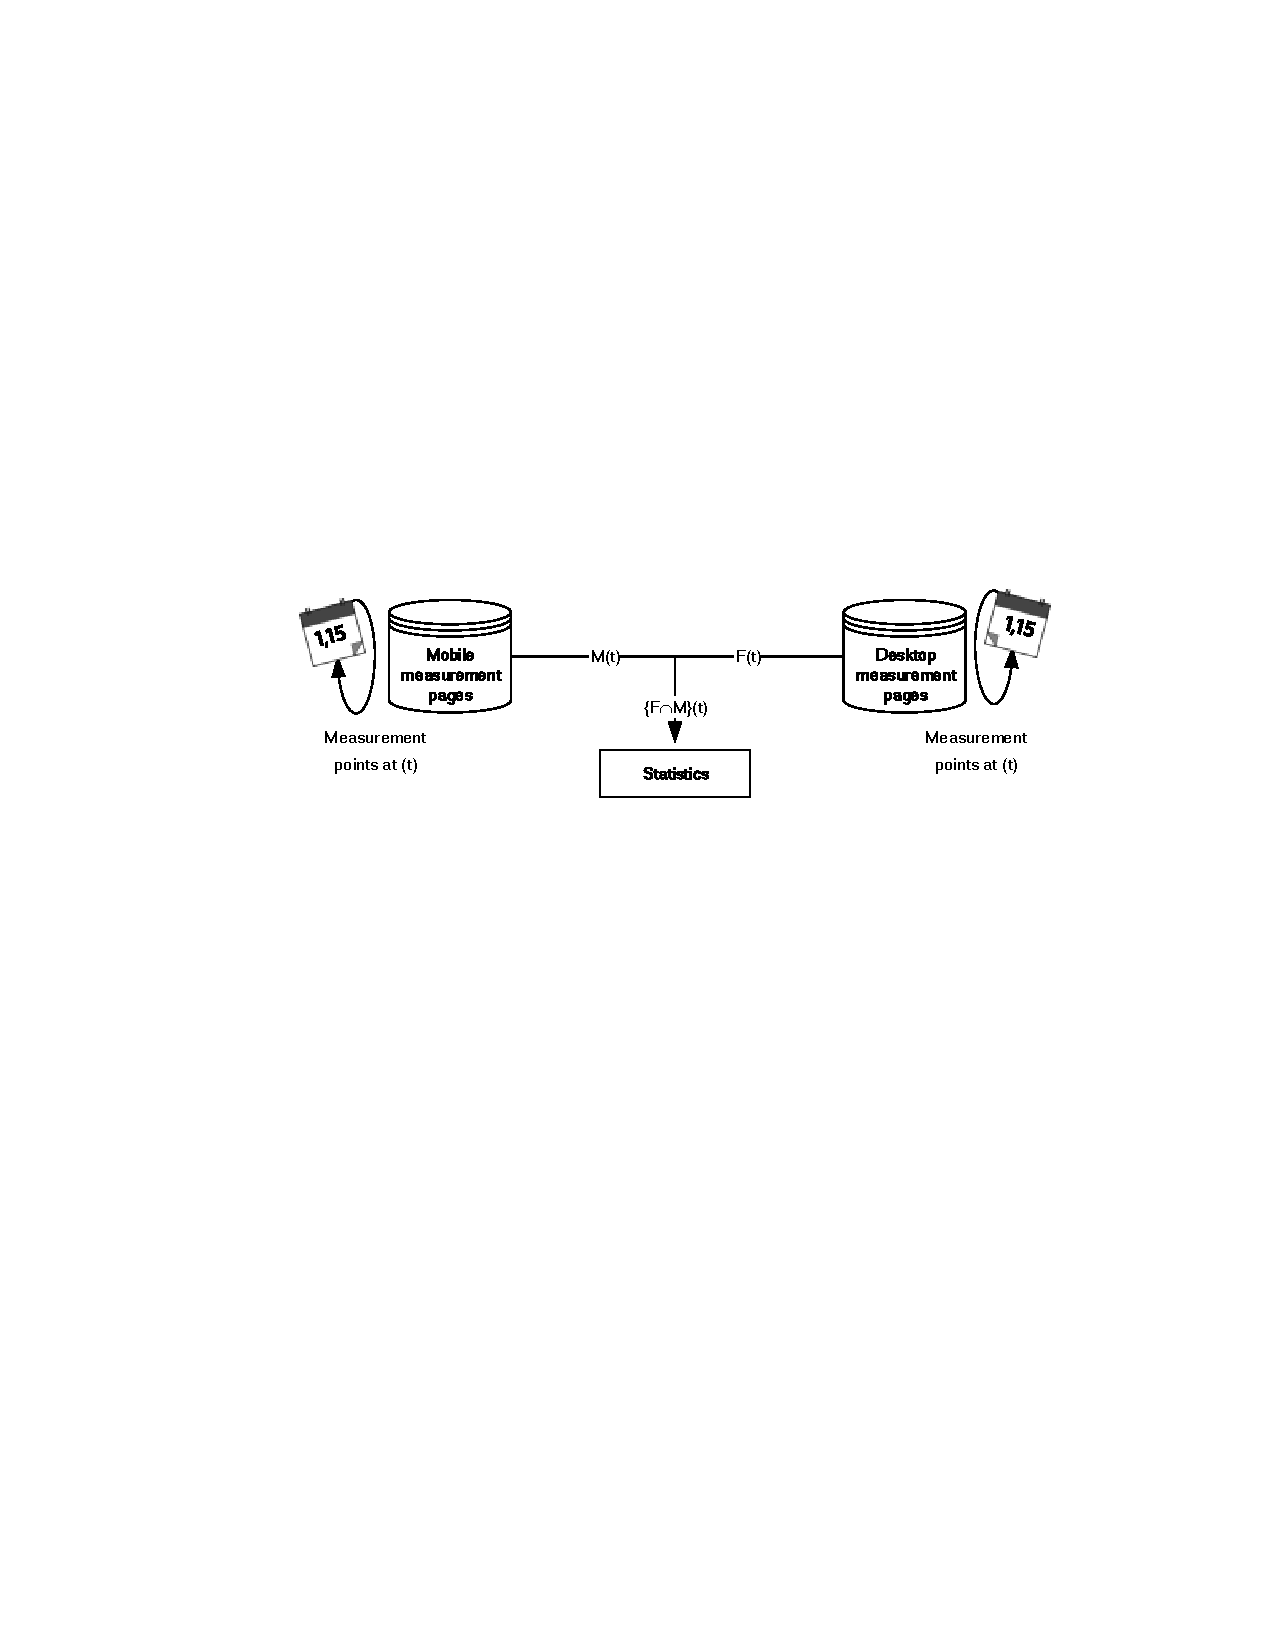
\includegraphics[width=.45\textwidth]{setup}
	\caption{Approach for gathering the general statistics evaluated in this contribution: based on the original archives, we compare the fixed and mobile web pages contained in each bi-monthly measurement and evaluate only those that can be found in desktop and mobile web page requests to allow for a direct comparison.}
	\label{fig:setup}
\end{figure}
As with any project that has to evolve over time to account for changes in technologies, some underlying measurement setups have to change over time as well.
In the remainder of this section, we describe the initial gathering and processing of this dataset in greater detail.


\subsection*{General Notes}
\addcontentsline{toc}{subsection}{General Notes}
As we utilize the measurements over a significant amount of time from June 1, 2011 to December 15, 2013, we initially note that some of the underlying measurement configurations have changed over time, which includes multiple facets, such as Unique Resource Locators (URLs), browser versions, connection speeds, or incorporation of `lazy loading' of resources.
We reason that overall, however, the changes made were reflecting industry trends as well as personal connectivity trends (such as modified access network speeds) and can be seen as representative of the typical connection scenarios for the World Wide Web.
We refer the interested reader to the online documentation of the \url{httparchive.org} project for more details pertaining to the measurement setup used and detailed information about changes.

\subsection*{Web Page Selection and Processing}
\addcontentsline{toc}{subsection}{Web Page Selection and Processing}
We select the available page statistics for both desktop (fixed) and mobile web pages over the range of more than two years; the available points in time are at the beginning and the middle of each month.
This results in a total of 62 datasets each for fixed and mobile web clients, respectively.
The evaluation by the httparchive.org project used the Apple iPhone's built-in browser client for mobile requests and the Microsoft Internet Explorer browser client for desktop requests (represented by different user agent strings in the HTTP requests sent).
We initially determine all web sites that are common for both archives, i.e., web sites that for each measurement time were evaluated for both, fixed and mobile clients, to allow for a comparative evaluation of their described metrics.
This results in a fair comparison at each individual measurement point, but yields an initial reduction of the total number of web pages that we compare. We note, however, that there are more than 900 pages in the initial (smallest) set. 
For each of the measurement times, we subsequently aggregate the measured web page characteristics over all web sites that were selected in a particular client role -- as a result, we derive a representative average snapshot of the characteristics that make up ``the web'' as accessed using different web clients over time.
In addition to the time-varying selection of web pages, we compare the web pages that are found for desktop and mobile clients throughout the longitudinal evaluation time period, which results in a smaller subset of 46 web pages.


\subsection*{Time Variability of the Dataset}
\addcontentsline{toc}{subsection}{Time Variability of the Dataset}
The underlying dataset that we utilize has undergone changes over time. 
Specifically, the base URLs that comprise the original dataset from httparchive.org (i.e., before we match fixed and mobile pages at each measurement point) were changed, namely ($i$) by switching to the Alexa top 1000000 web sites in November 2011 and ($ii$) by increasing the number of URLs evaluated in September 2012, see~\cite{ht13}. Other changes that were performed are more network-level oriented and should have a lesser impact on the static results we report here.
To evaluate how these changes impact the diversity of values encountered in the dataset over time, we employ the entropy of the Theil population, which is itself based on the Theil index~\cite{Th72}.

Specifically, we evaluate the number of web requests and the total number of bytes for each request type over time, as we are more interested in the overall quality of the selected data subset (i.e., statistics for pages that can be found in both datasets).
We illustrate the result as function of time in Figure~\ref{fig:theil}, whereby we initially note that higher values represent a higher diversity of the underlying dataset (Theil population).
\begin{figure}[t]
	\centering
	\subfloat[Number of requests per page]{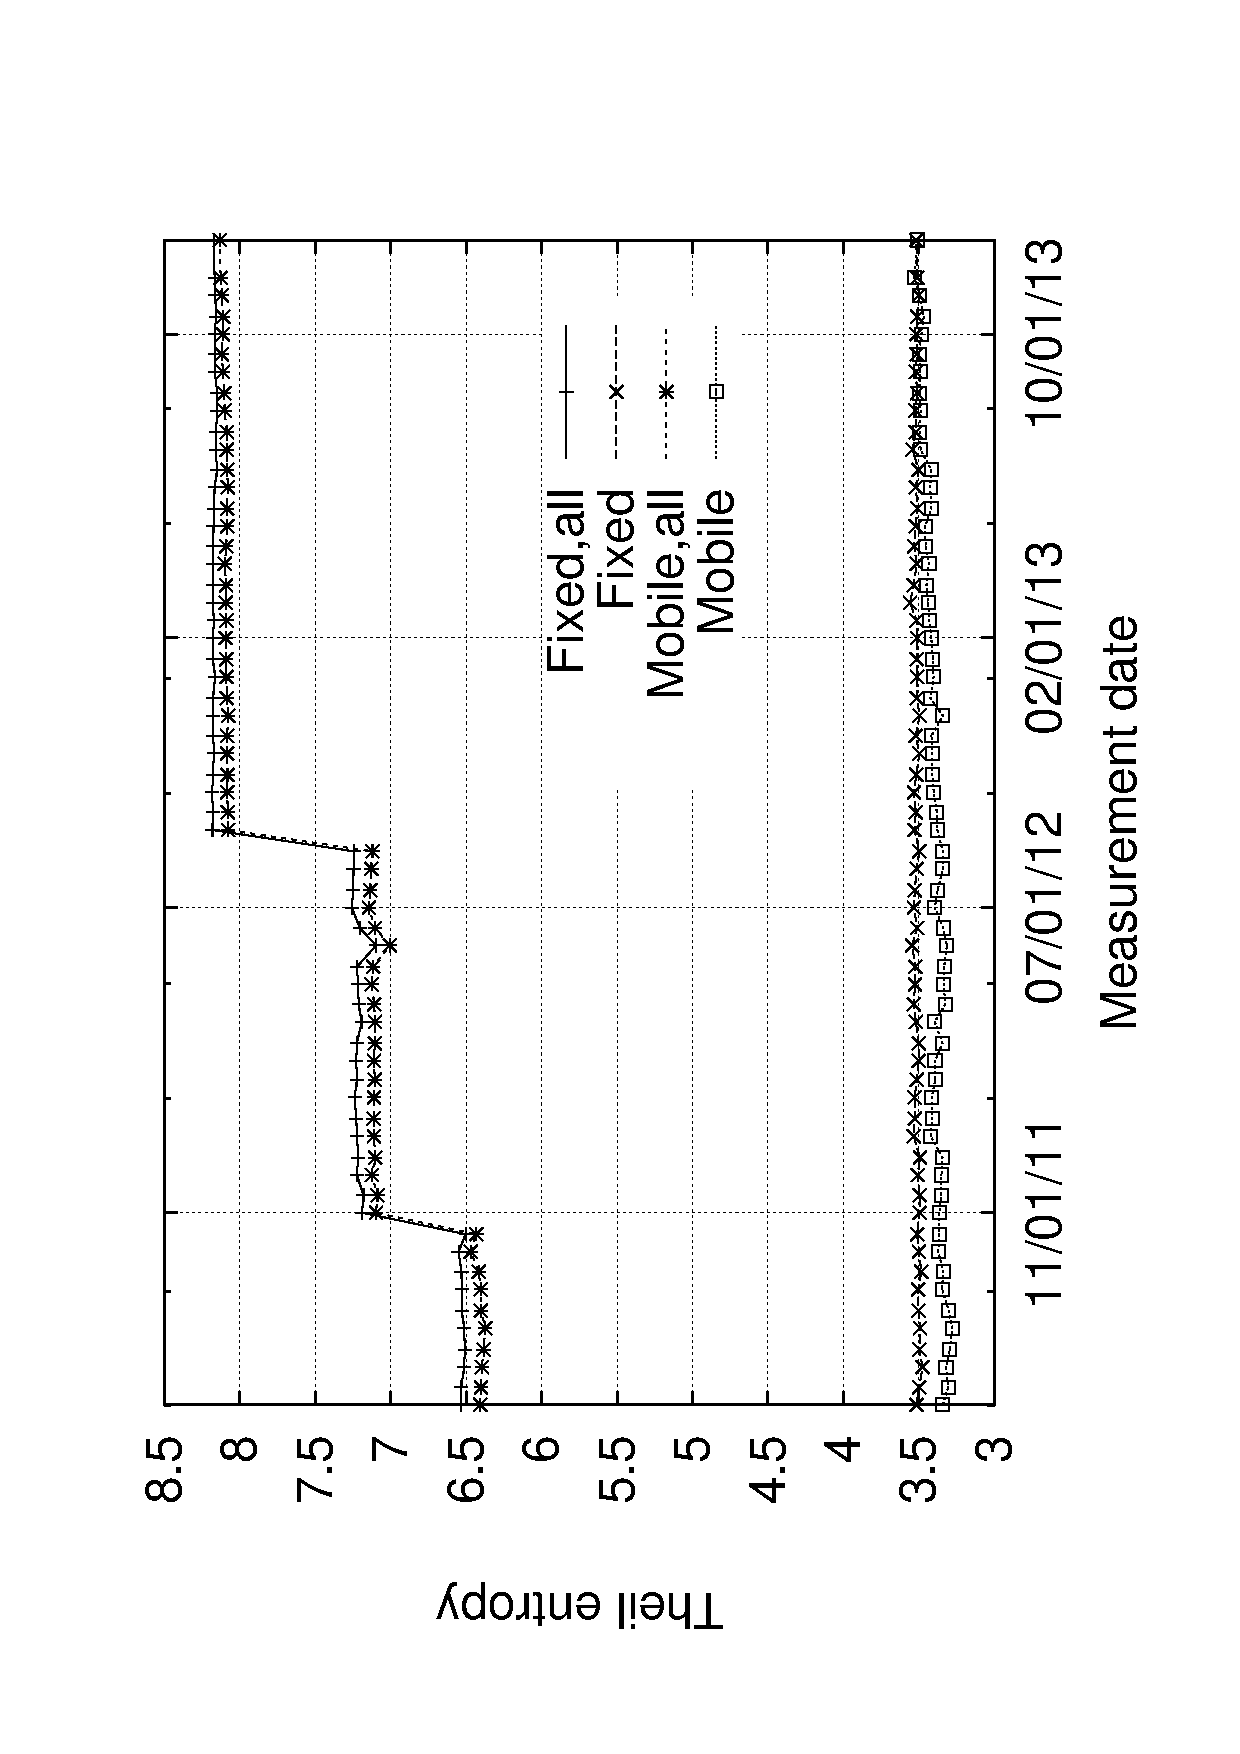
\includegraphics[width=.45\textwidth]{theil_reqs}}\qquad
	\subfloat[Number of bytes per page]{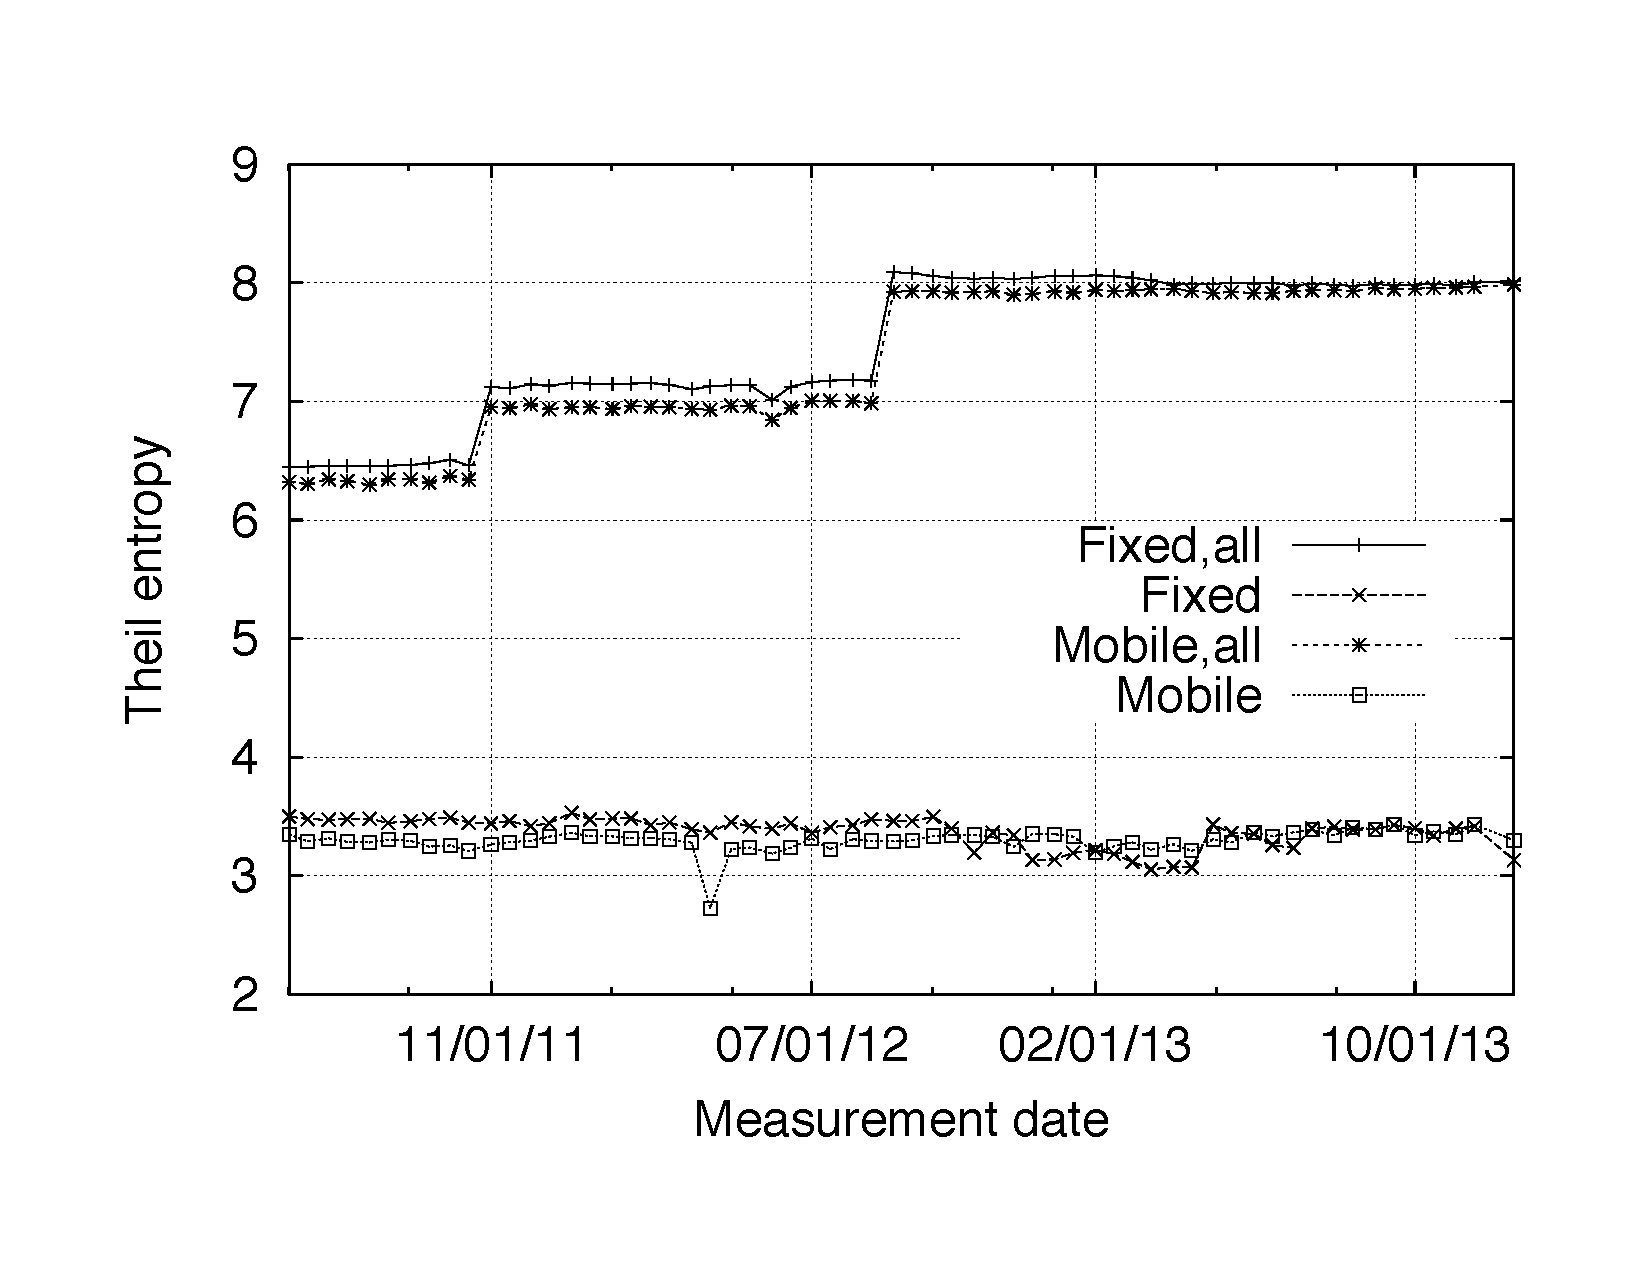
\includegraphics[width=.45\textwidth]{theil_bytes}}
	\caption{Theil entropy for the number of objects requested and the number of bytes for web pages present in the httparchive.org's desktop and mobile client data files for all pages at each measurement point (all) and the subset of continuously included pages.}
	\label{fig:theil}
\end{figure}
We observe that the entropy curves for each of the selected features (requests, bytes) are fairly close for each of the two modes (fixed, mobile), with significant ``jumps,'' i.e., changes of their overall level, at two distinct measurement points for the larger dataset.
These ``jumps'' occur at times where the underlying number and source set of the httparchive.org base URLs were changed, as outlined above.
We note that these changes, however, affect all client modes and type of characteristics evaluated in a similar manner by significantly increasing the diversity of measurement results, which is immediately visible from Figure~\ref{fig:theil}.
For the smaller subset, we observe a more steady behavior, with only small deviations and outliers over the entire measurement time period.
Overall, we note that the Theil entropy levels for the desktop client values are slightly higher than their mobile client counterparts; however, they remain within close range.
This closeness in the calculated Theil entropy additionally motivates us to focus on the overall averages of the values we compare in the remainder of this paper.


\section*{Comparison of Desktop and Mobile Web Page Characteristics}
\addcontentsline{toc}{section}{Comparison of Desktop and Mobile Web Page Characteristics}
\label{s:compare}
In this section, we compare the average values we obtained from the joint httparchive.org datasets for the desktop and mobile web client versions of the same set of web pages requested, as given by their URLs.

\subsection*{Average Number of Web Site Objects}
\addcontentsline{toc}{subsection}{Average Number of Web Site Objects}
\label{ss:objects}
Initially, we investigate the average number of objects requested when accessing a web page for the first time and illustrate the results in Figure~\ref{fig:requests} for both client types and all web pages compared to the subset present throughout all measurement points.
\begin{figure}
\centering
	\subfloat[Average requests for desktop and mobile client versions.]{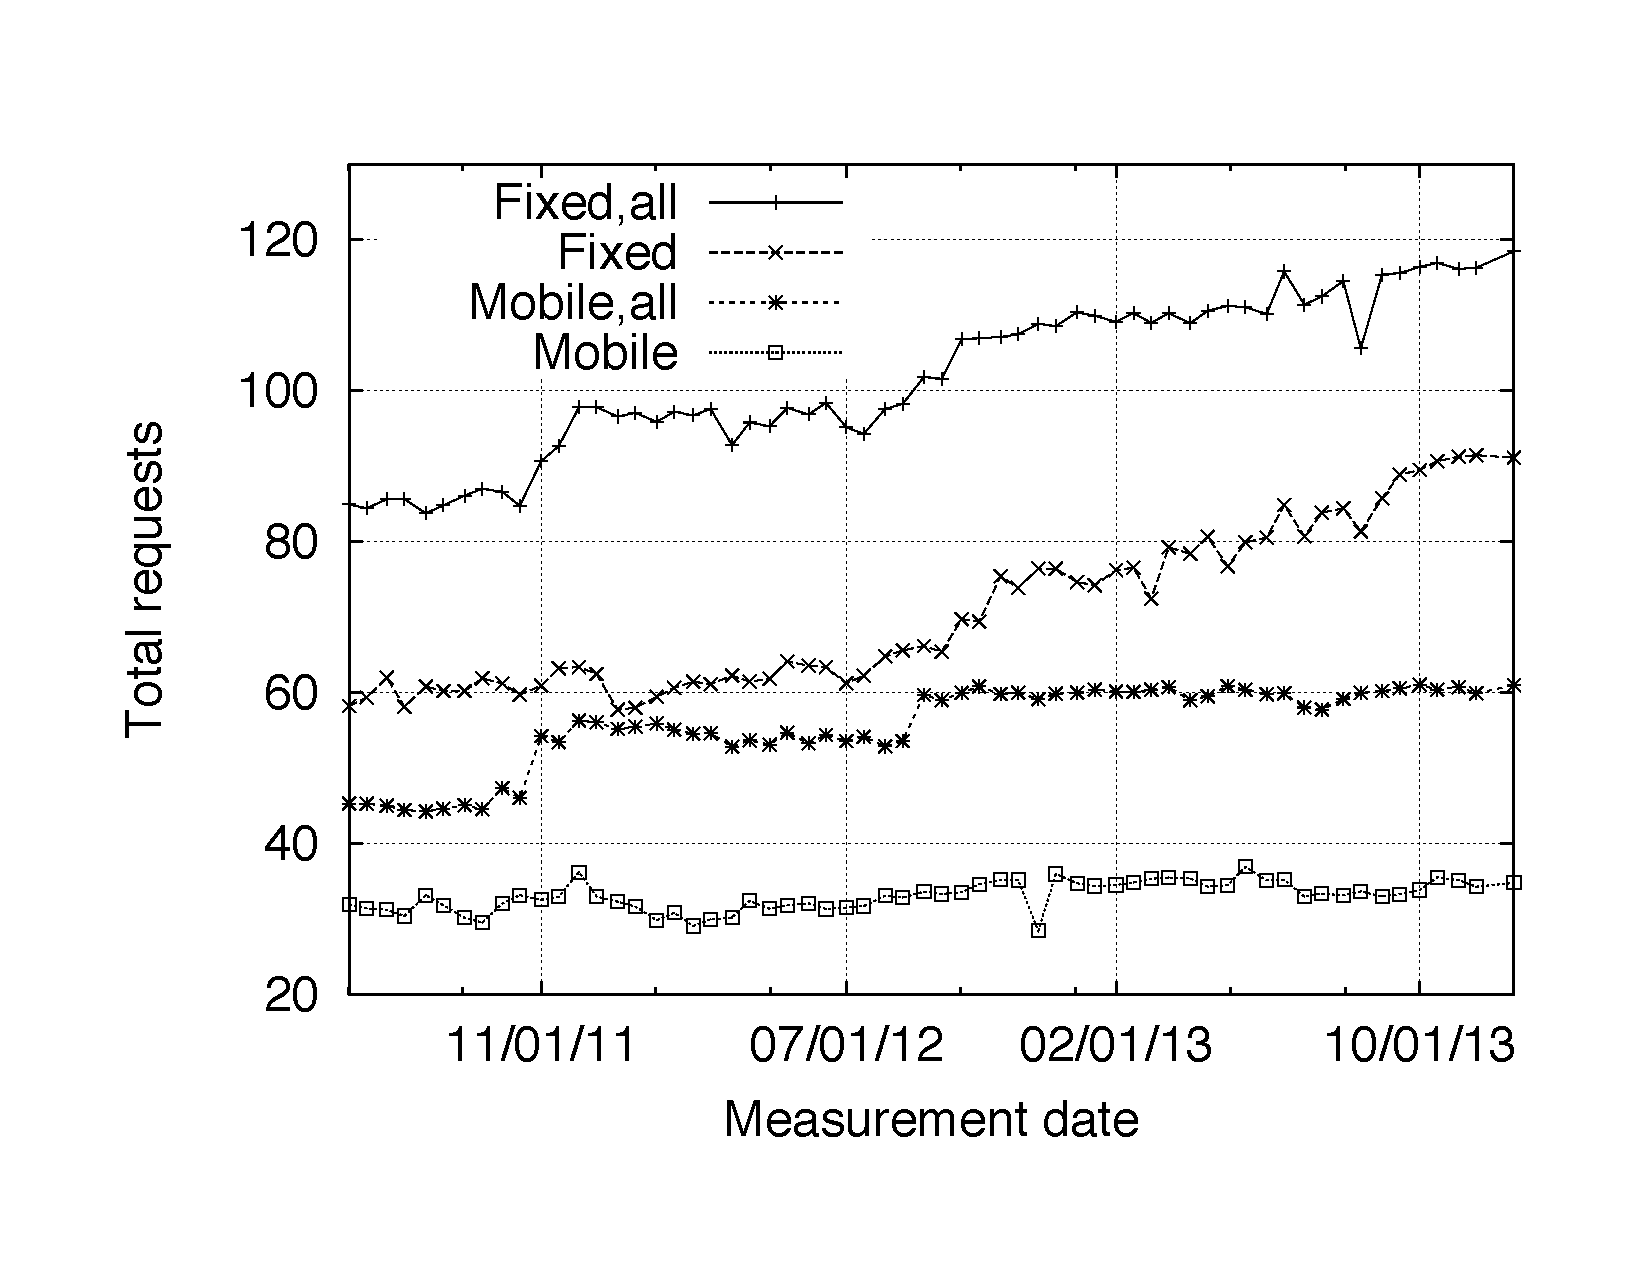
\includegraphics[width=.45\textwidth]{totalRequests_all}}\\ 
	\subfloat[Categorized requests for desktop client (all pages).]{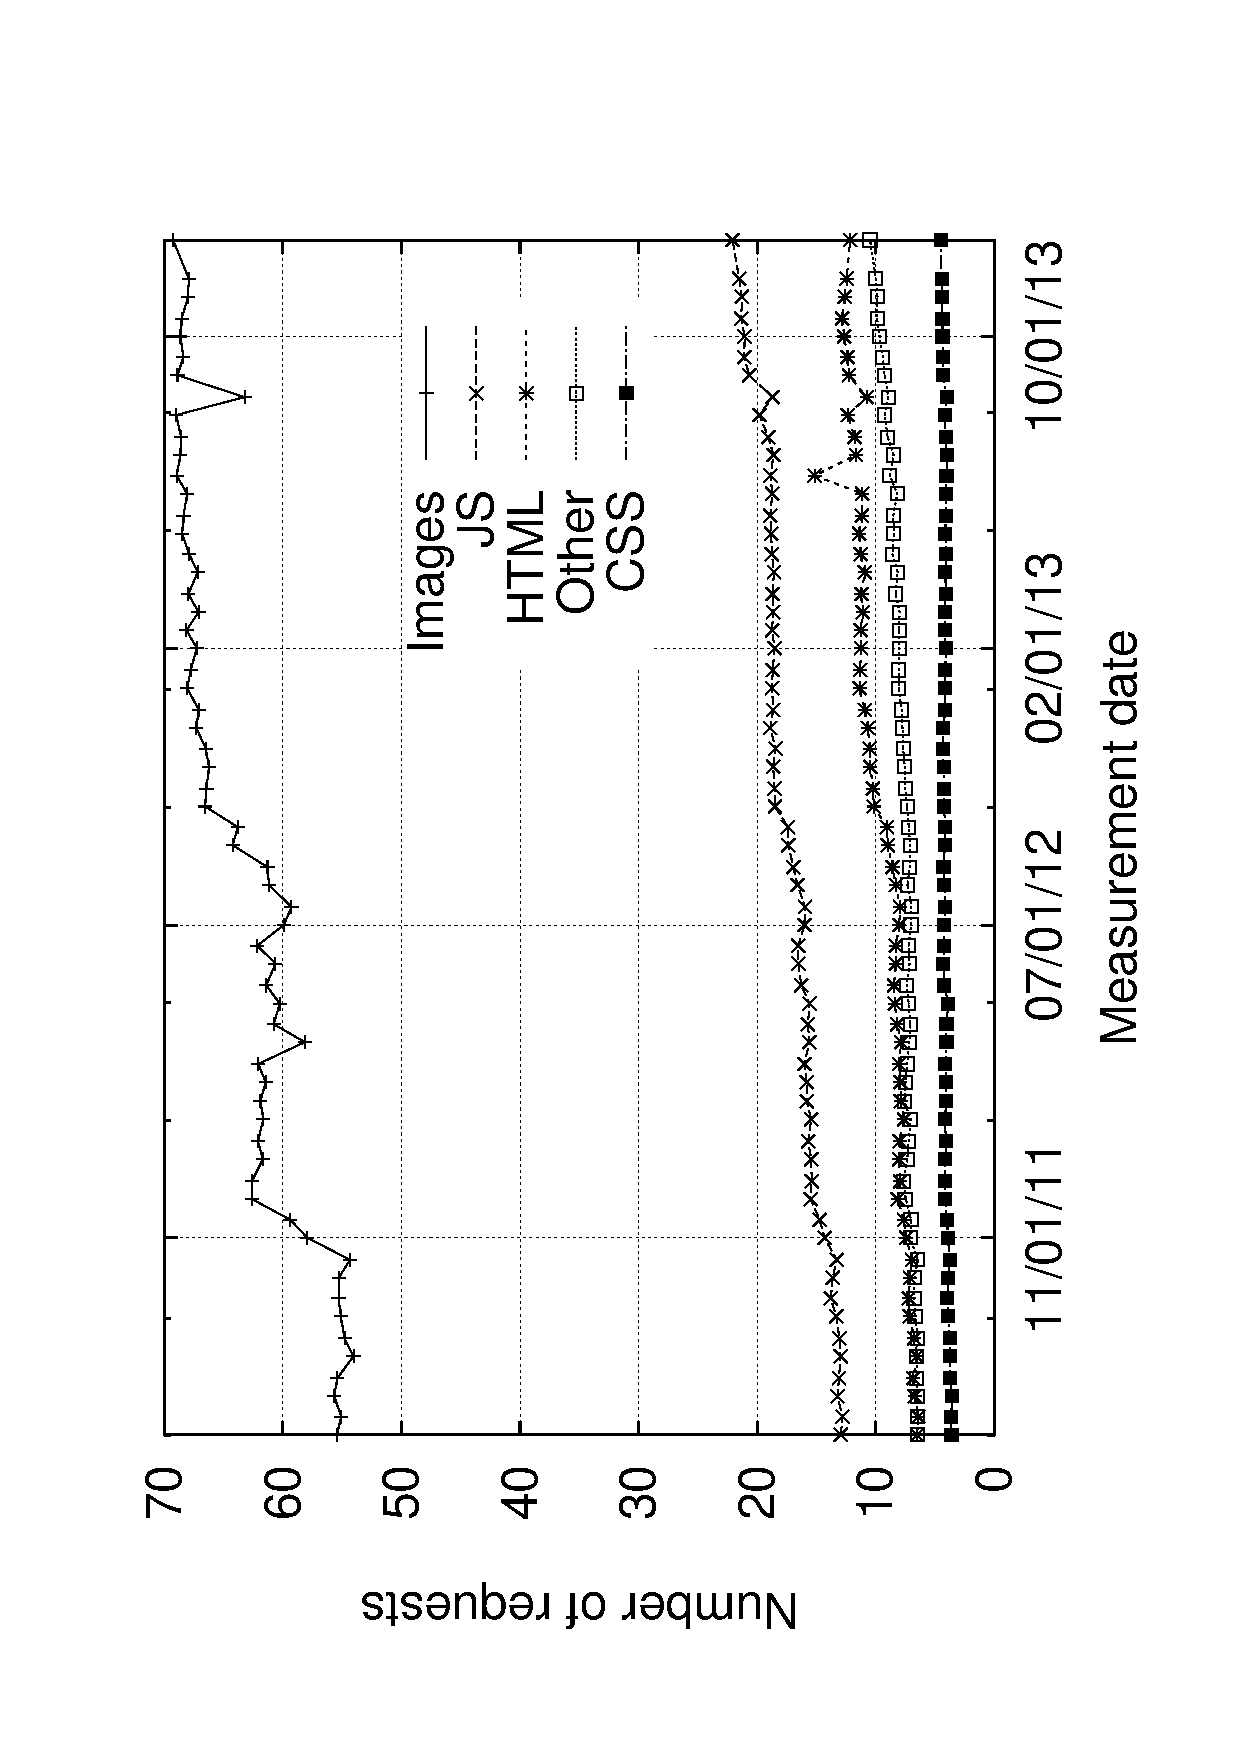
\includegraphics[width=.45\textwidth]{req_by_type_fixed_all}}\qquad
	\subfloat[Categorized requests for mobile client (all pages)]{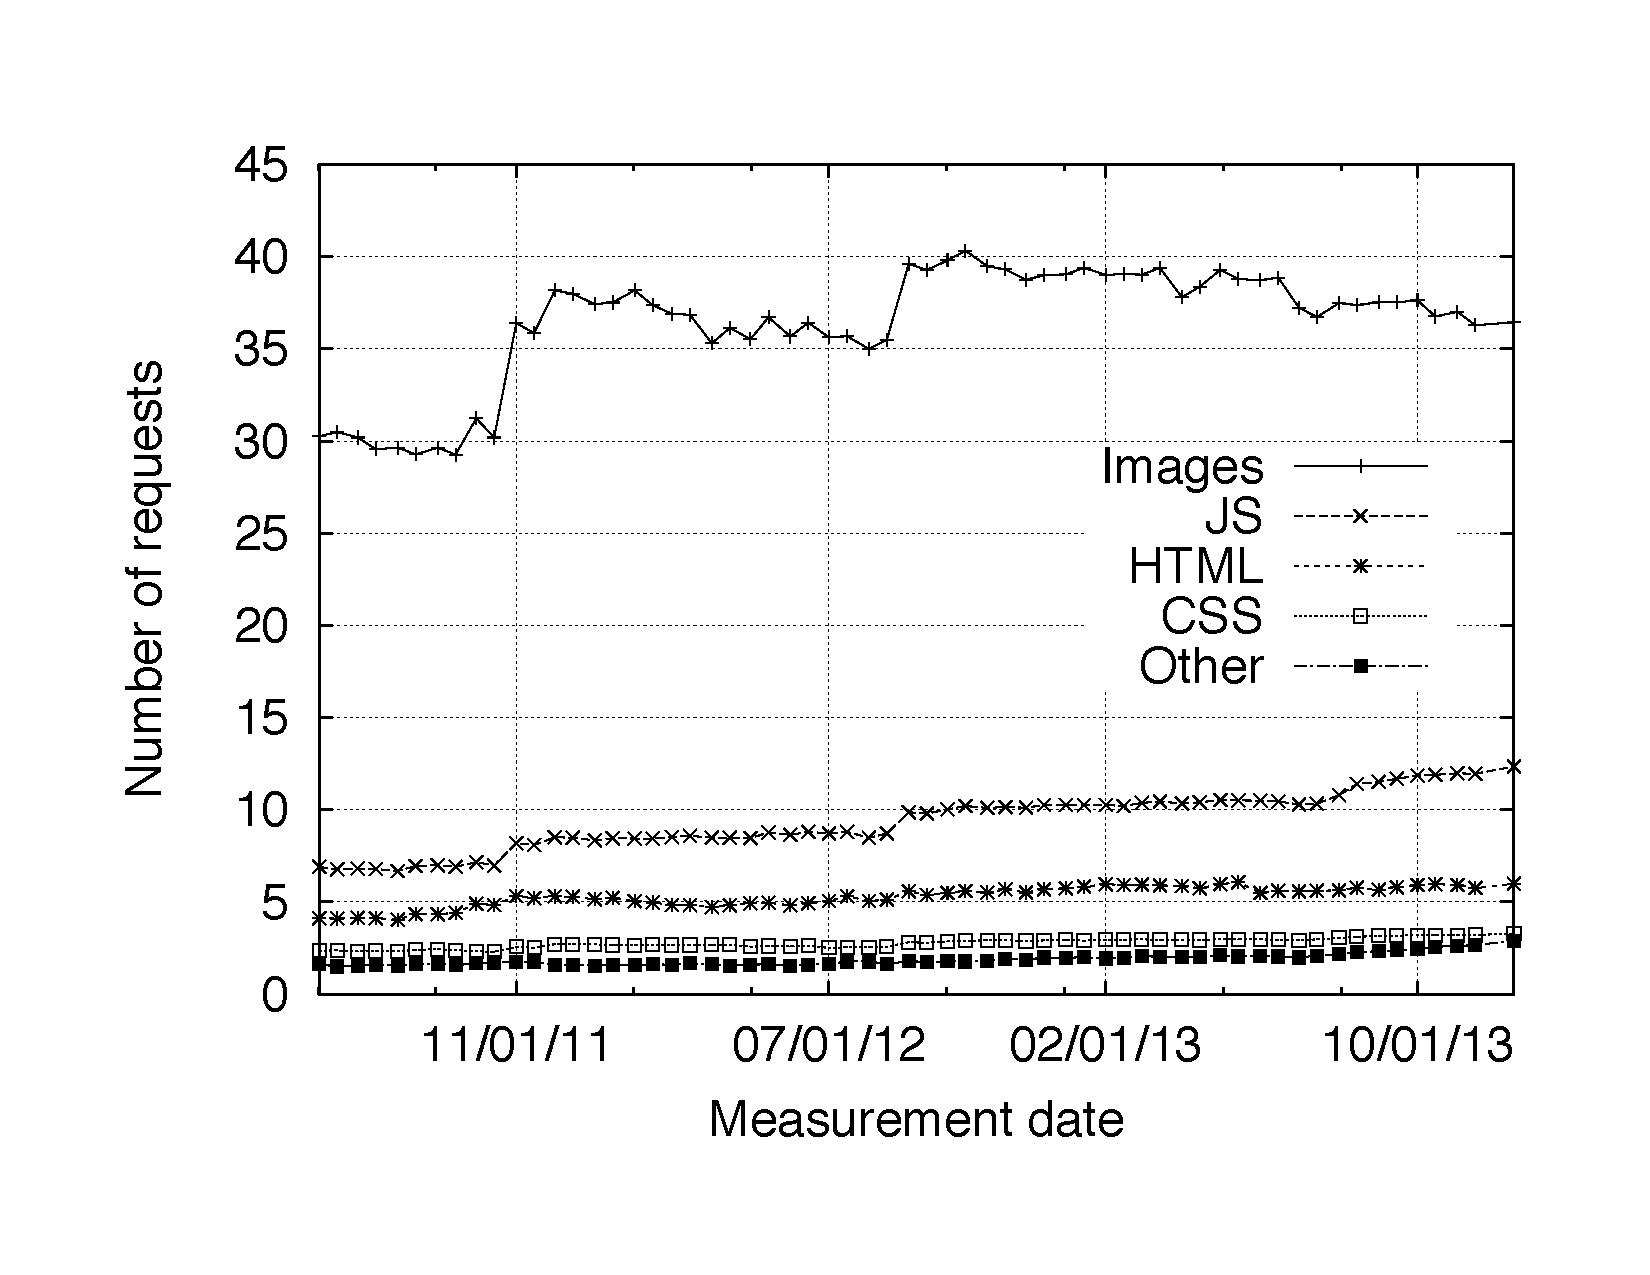
\includegraphics[width=.45\textwidth]{req_by_type_mobile_all}}\qquad
\caption{Average total number of requests for objects constituting a web page in desktop and mobile versions and decomposition into  HTML, CSS, Java Script, Images, and Other object categories.\label{fig:requests}}
\end{figure}
We initially note that the desktop versions exhibit a significantly larger number of requested objects in comparison to the mobile counterparts.
We additionally observe an overall continuous increase, which tends to have slight ``jumps'' in certain time frames (more pronounced for mobile client requests). 
These slight increases are in line with the earlier observations concerning changes to the underlying web pages constituting the measurement points in time. While significant variability between individual measurement points can be noted,  the overall trend remains steady and slowly growing.


Most notably, we witness the increase to over 100 requests on average per web page requested by a desktop client and its continued growth since the second half of 2012.
Within the same time period in 2012, the mobile web request counterpart rose to over 60 requests, with a steadily trend thereafter. 
We compare these trends for all web pages at each measurement point with the continuously present subset in Figure~\ref{fig:requests}~(a) as well.
We note that the web pages of the subset exhibit significantly lower levels of the average number of requests per web page for both versions. 
When evaluating the overall trends, however, we find that the subsets exhibit similar ones, hence corroborating our earlier observations for all pages.

Investigating the origins of the average number of web object requests in greater detail, we illustrate the composition of the average number of objects requested separated into the categories of HTML, CSS, Java Script, Images, and Other objects over time in Figure~\ref{fig:requests}~(b) for desktop client requests.
The Other category contains items such as fonts, Flash elements, as well as any remaining downloaded web page components.

We initially observe a rising trend for all categories, with the image category accounting for the most requests and the remaining ``other'' category continuing somewhat steady over time.
Keeping the overall increasing trend in mind, we note the distribution between the different categories of objects remains rather steady over time (with categories in desktop client requests accounting for approximately the following long-term averages: Images 74\%, Java Script 19\%, HTML 11\%, Others 9\% , and CSS 5\%).
For mobile requests, on the other hand, we observe in Figure~\ref{fig:requests}~(c) a nearly identical order at a lower level (with categories in mobile client requests accounting for approximately the following long-term averages: Images 80\%, Java Script 20\%, HTML 11\%, CSS 6\%, and Others 4\%).
We note that an evaluation of the categorized average number of requests per web page yields similar results for the subset of pages (omitted due to space constraints).

We conclude from these numbers that for both scenarios, the main culprit for web requests is provided by the images contained in web sites, and to a lesser extent the oft-mentioned Java Script, found in modern AJAX and HTML5 based pages in fixed as well as mobile environments.

\subsection*{Average Web Page Sizes}
\addcontentsline{toc}{subsection}{Average Web Page Sizes}
\label{ss:bytes}
We now shift our view to the average sizes of desktop and mobile client requested web pages over time as well as their most contributing factors.
We initially illustrate the total number of bytes that were required on average to download a web page to a fixed and a mobile client in Figure~\ref{fig:sizes}.
\begin{figure*}
	\centering
	\subfloat[Averages for desktop and mobile client versions.]{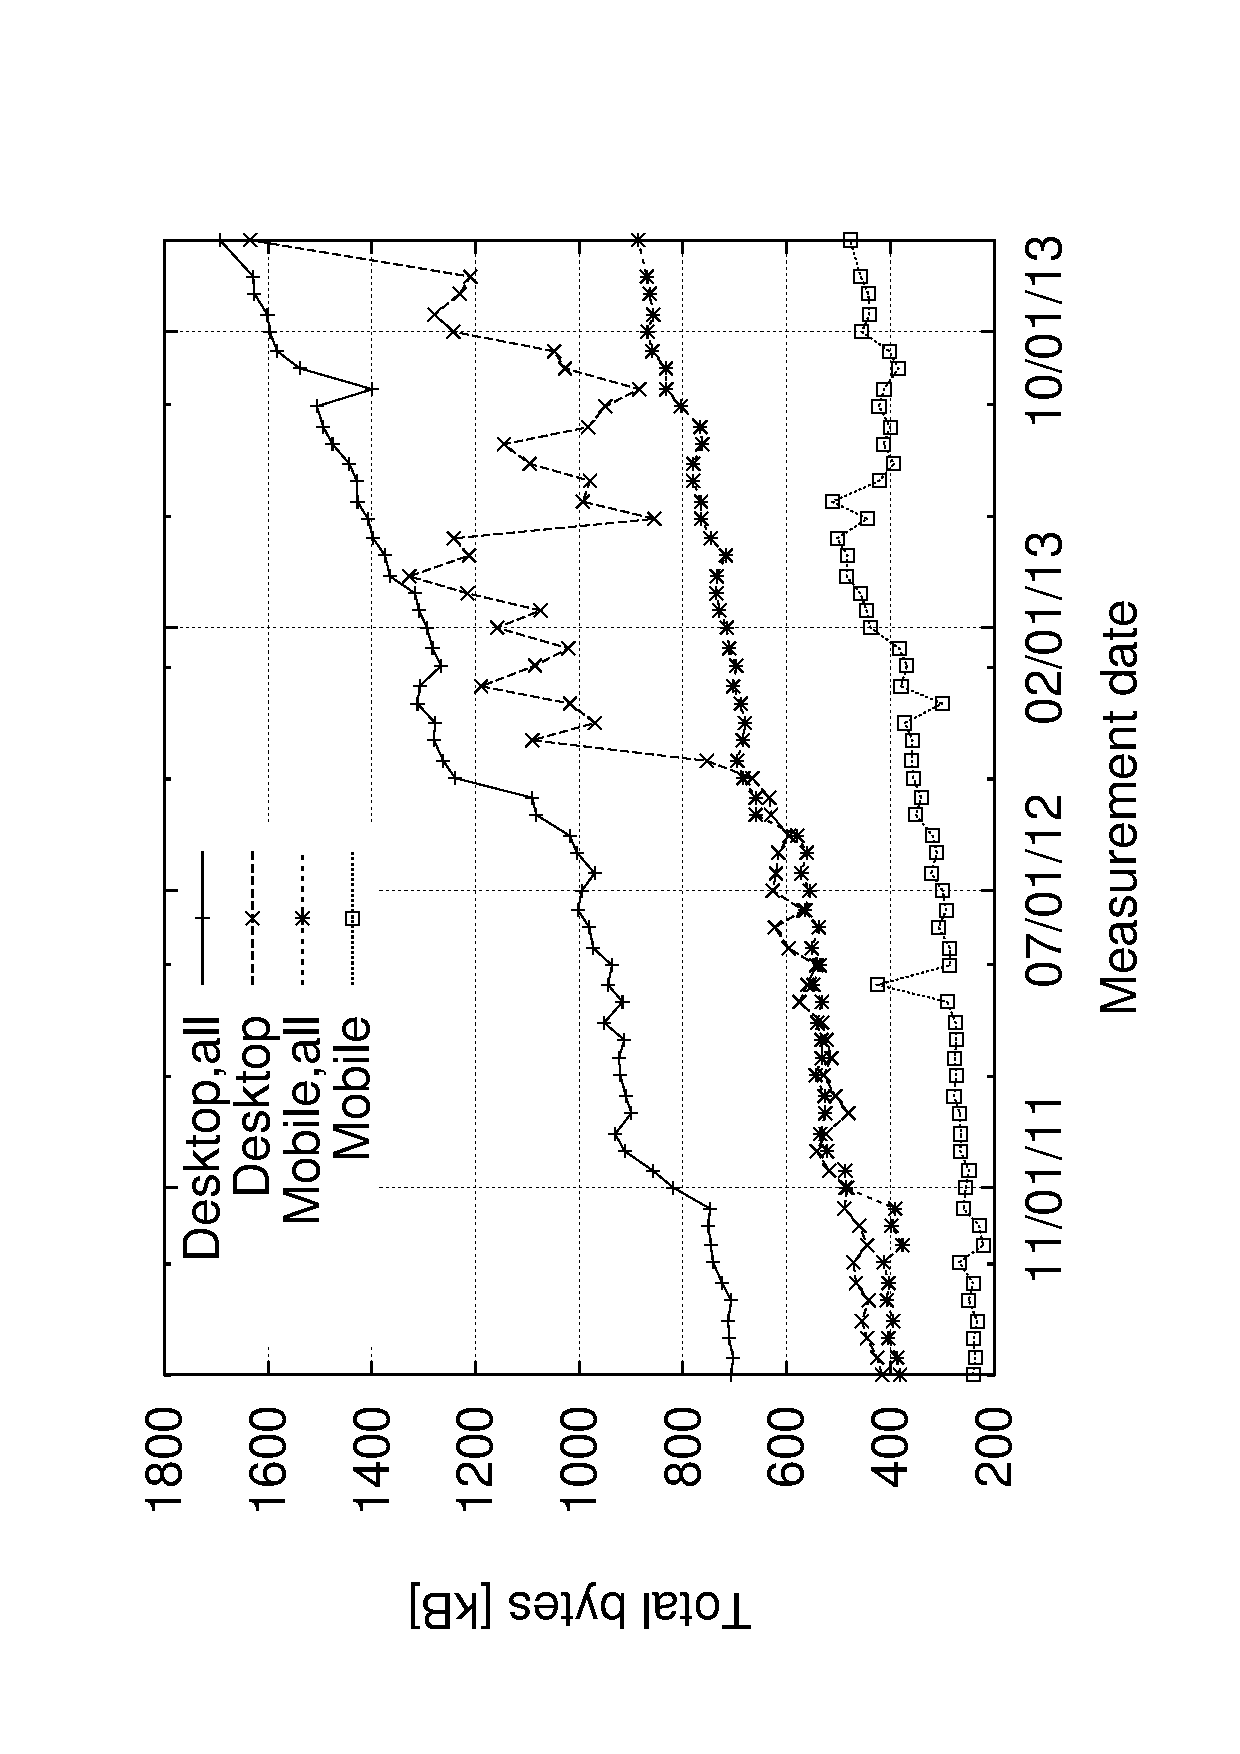
\includegraphics[width=.45\textwidth]{bytes_total_all}}\qquad
	\subfloat[Categorized for desktop client (all pages).]{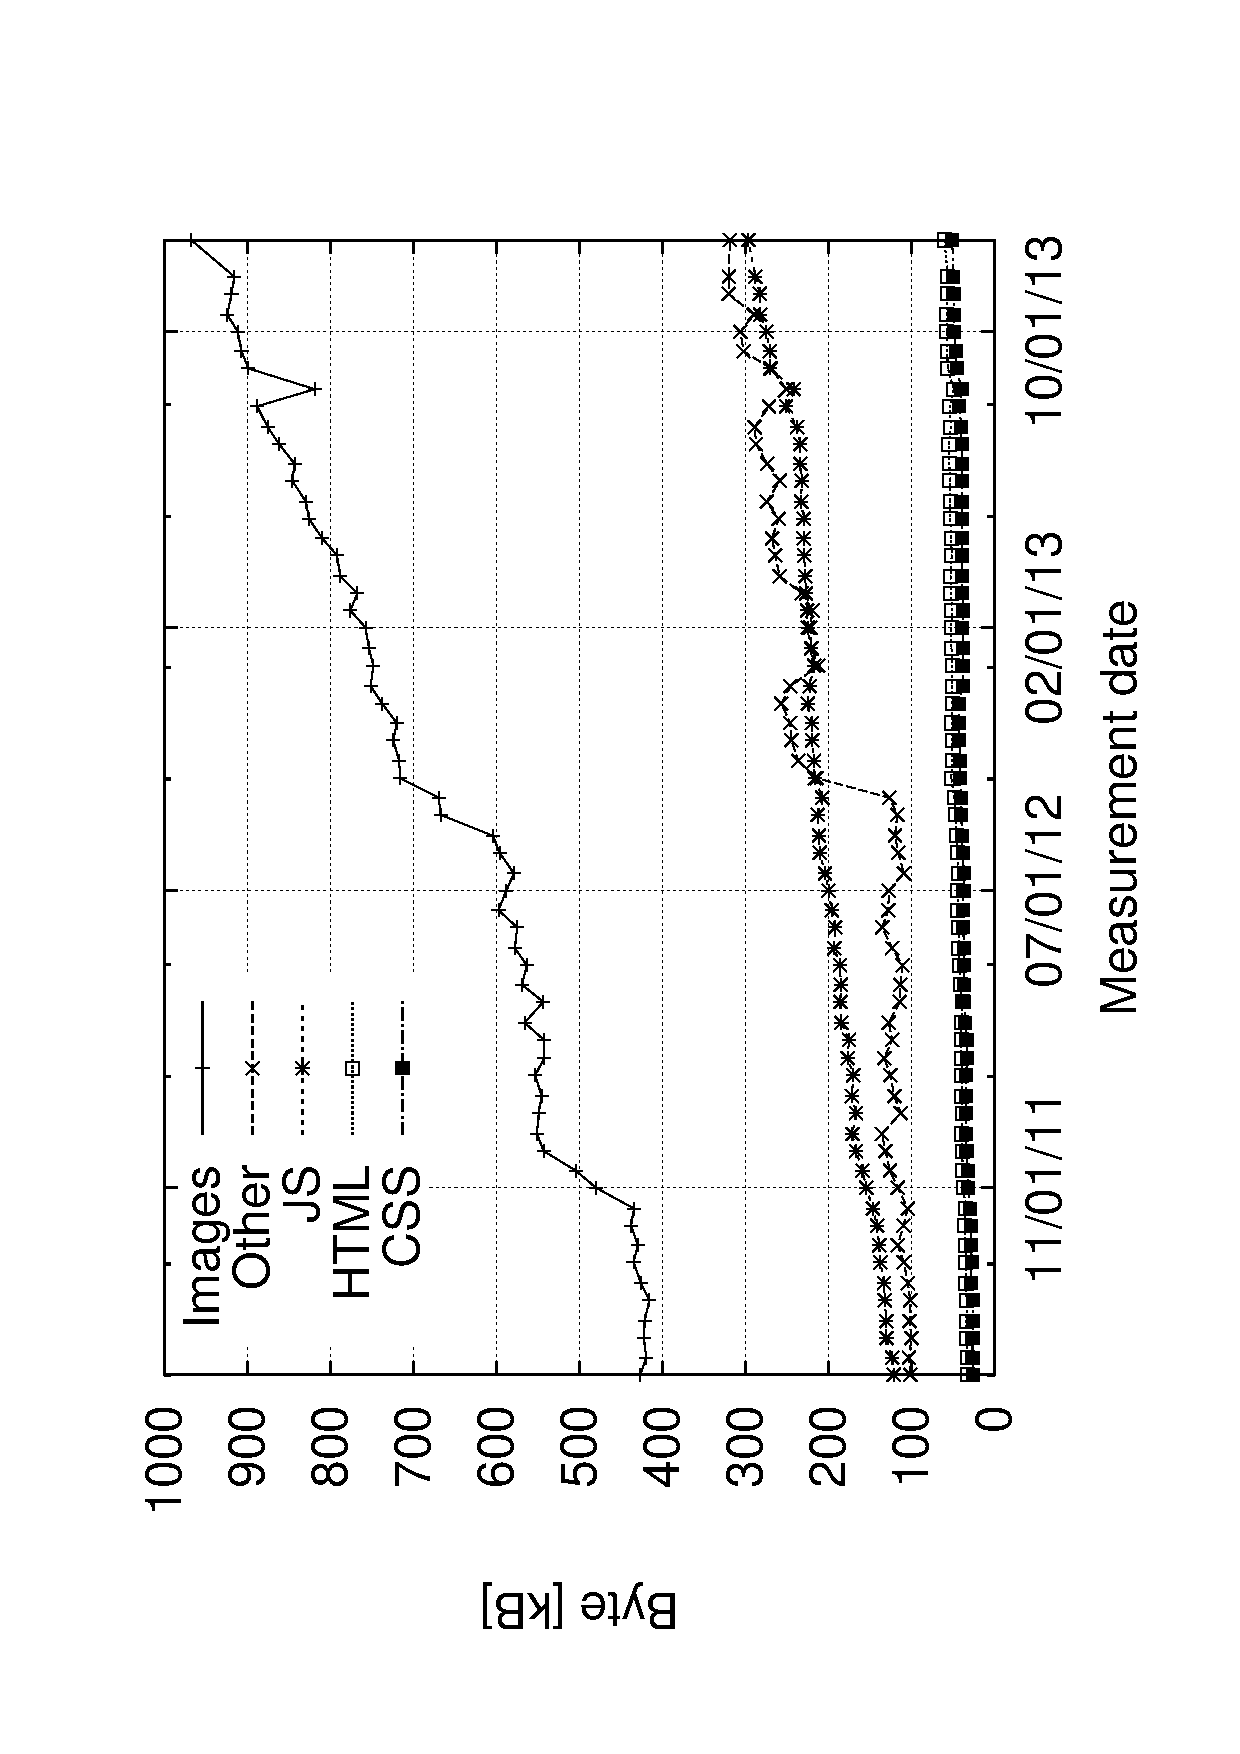
\includegraphics[width=.45\textwidth]{bytes_by_type_fixed_all}}\\
	\subfloat[Categorized for desktop client (subset).]{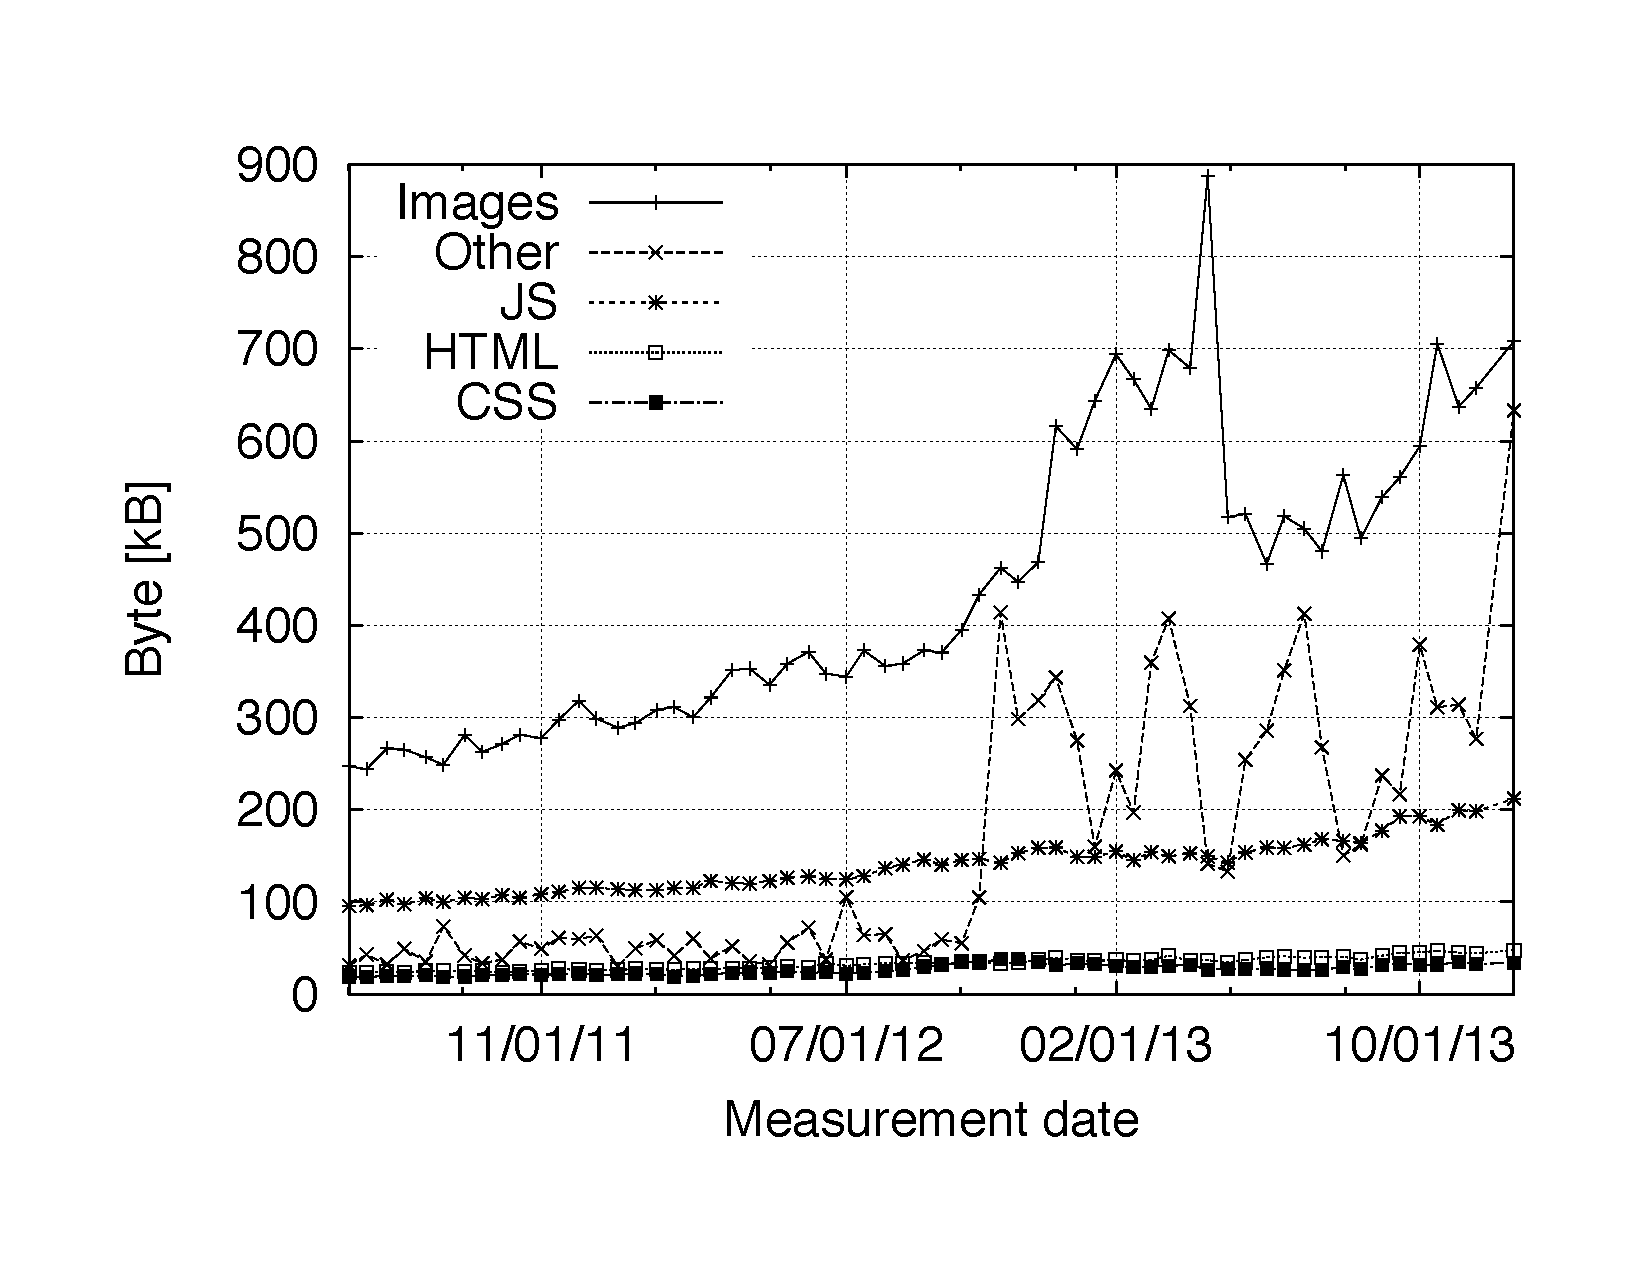
\includegraphics[width=.45\textwidth]{bytes_by_type_fixed}}\qquad
	\subfloat[Categorized by category for mobile client (all pages).]{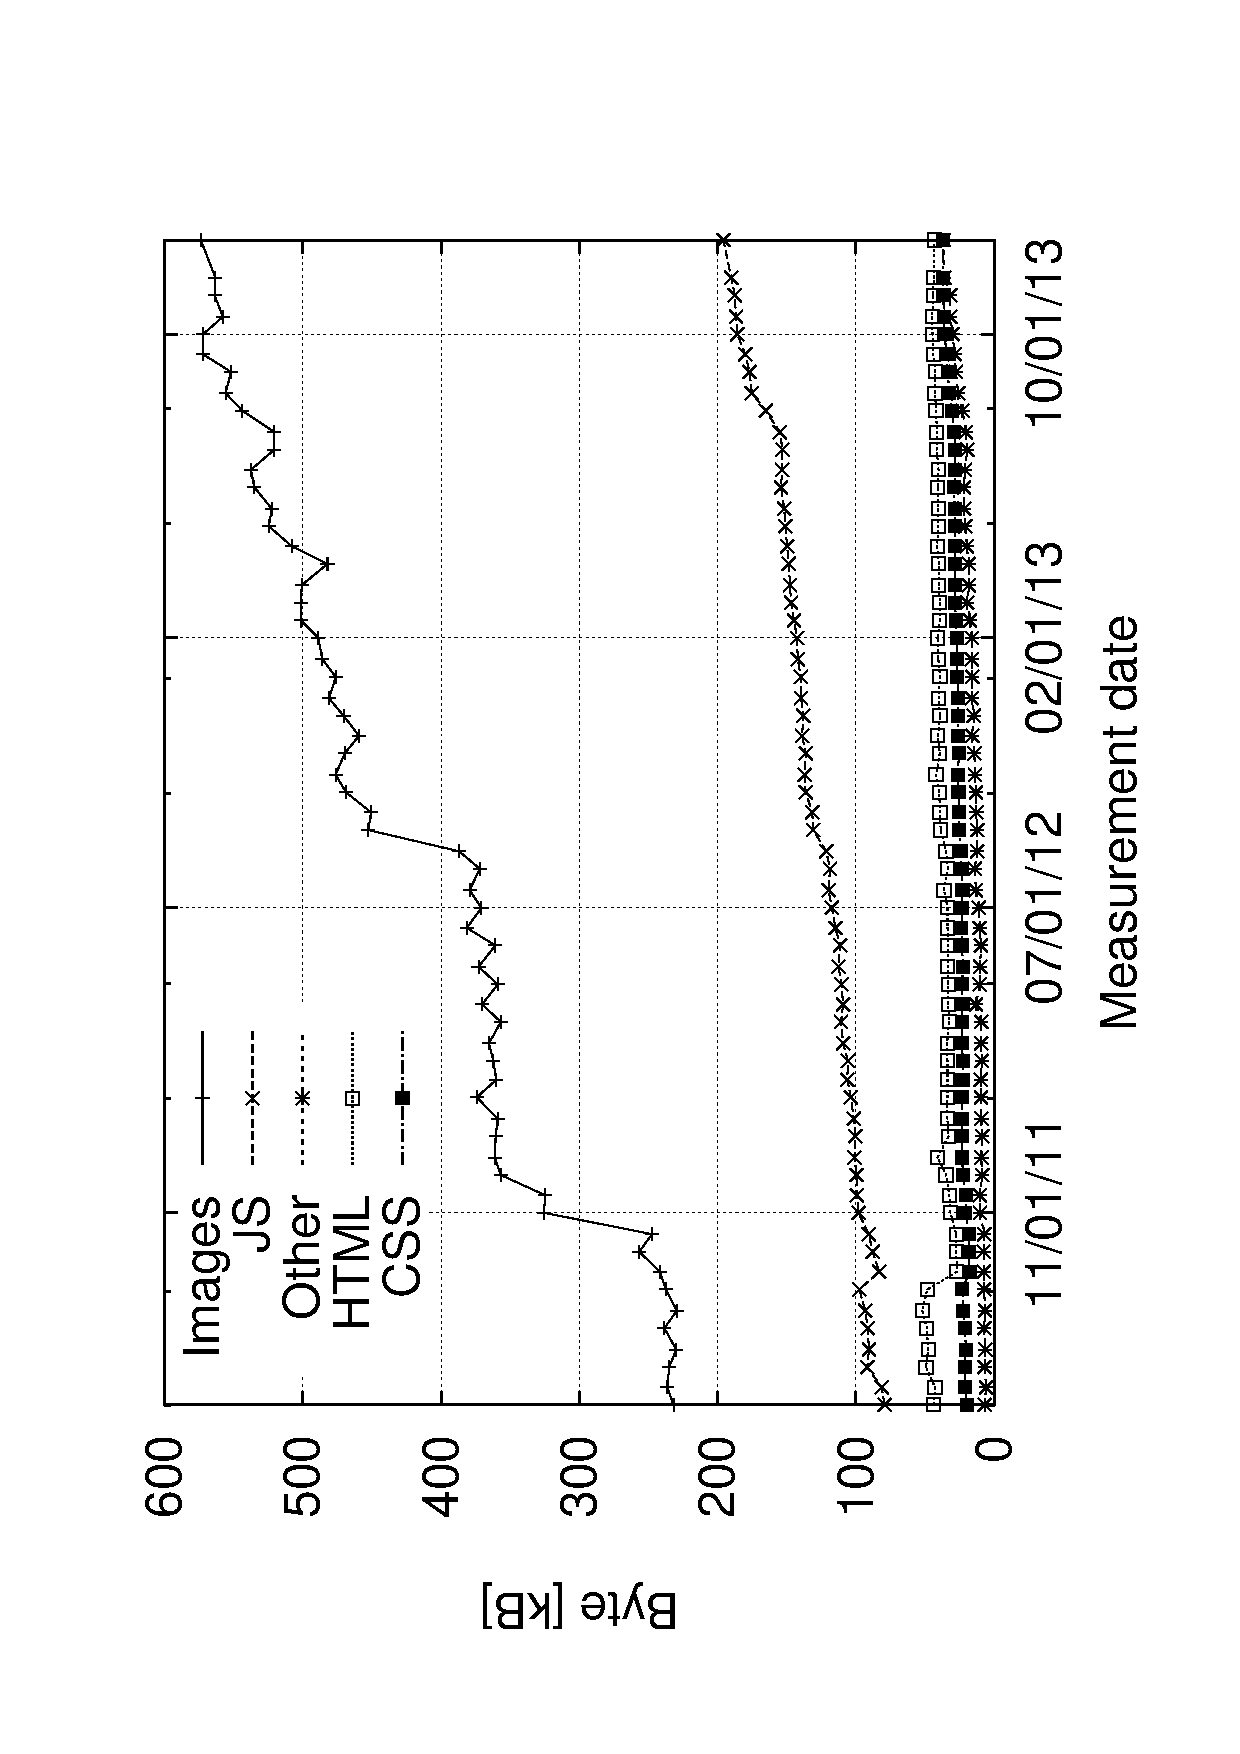
\includegraphics[width=.45\textwidth]{bytes_by_type_mobile_all}}\qquad
	\caption{Average total number of bytes constituting a web page in desktop and mobile versions and decomposition into  HTML, CSS, Java Script, Images, and Other object categories.\label{fig:sizes}}
\end{figure*}

We observe that the fixed sizes are always larger than their mobile counterparts and that both continuously increase over time. 
This leads to the average web page size to have increased from 0.71 MB in June 2011 to over 1.5 MB in December 2013 for desktop client and from 0.38 MB to almost 0.9 MB for the mobile counterparts in the same time frame.
In greater detail, we note that the average increase in average web page sizes over time for fixed web pages during the evaluated time period is around 3\% per month or approximately 41\% per year, while the mobile counterparts feature an increase of 3\% or 40\%, respectively.
We also find that the average mobile web page sizes currently trail their desktop counterparts by approximately 1.75 years, which likely will increase due to the difference in average growth rates (1.57\% vs. 1.47\% on average in every two week time period for fixed and mobile web pages, respectively).
Similar to the average number of requests, we compare the subset of 46 web pages to the complete dataset in Figure~\ref{fig:sizes} as well.
We observe a similar behavior here with the subset's reduced average number of bytes for the first half of the observation period. In the second half, the fixed web pages exhibit a significant increase in the average sizes and variabilities thereof. 
However, the overall rising trend is present for both versions and corroborates our overall rising trend observations.

Investigating the origins of the average number of web page sizes, we illustrate the composition of the average number of bytes requested separated into HTML, CSS, Java Script, Images, and Other object categories over time in Figure~\ref{fig:sizes}~(b) for desktop client requests.
We immediately note that while all components are increasing in size over time, the main contributors to the growth are the Images and Other web page object categories.
More specifically, we note that the three main contributors to total web page sizes are images, other components, and Java Script. 
While the number of bytes contributed by Java Script has slowed in growth, images (which have almost doubled in the number of bytes) and other web page items (which more than doubled) continue their growth over time.
We can attribute this behavior to the richer web experience that users demand, with additional interactivity and visually stimulating appearance.
HTML and CSS components of web pages, on the other hand contribute only a minimum amount of data, with little increase over time.
Comparing the detailed categorized values with the subset of web pages in their desktop versions, we note that the origin of the radical increase in average sizes can be attributed to the increase of data in the images and other categories.
Some of these individual spikes can be attributed to individual outliers, such as a handful of web pages exhibiting very large object sizes. On http://www.tumblr.com on April 15, 2013, an approximate 15 MB image was encountered, which can be seen as anecdotal representation of automated processes (such as the background image for that particular homepage being picked from user posts) lacking optimization routines (such as downscaling in this case).


Shifting the view to the average sizes of the web page components for mobile clients, we also note an overall growth trend for all categories as illustrated in Figure~\ref{fig:sizes}~(d).
For mobile clients, however, the overall average web page sizes stem mainly from images and secondly Java Script. 
The remaining three categories contribute significantly less data and exhibit a slower growth.
It is interesting to note from comparison with the desktop counterparts, that the average mobile client image sizes are approximately two thirds of their desktop counterparts.
Unlike the average number of requests, however, the average number of bytes clearly identifies Java Script for mobile devices as one of the main causes of increased web page sizes. 
We exclude the detailed evaluation of the subset's characteristics here, as the results resemble earlier observations and their conclusions.


\subsection*{Data per Web Page Object}
\addcontentsline{toc}{subsection}{Data per Web Page Object}
Combining the two former evaluations, we now evaluate the average web page object request size.
We illustrate the overall and categorized views in Figure~\ref{fig:relative}.
\begin{figure}[]
	\centering
	\subfloat[Averages for desktop and mobile client versions.]{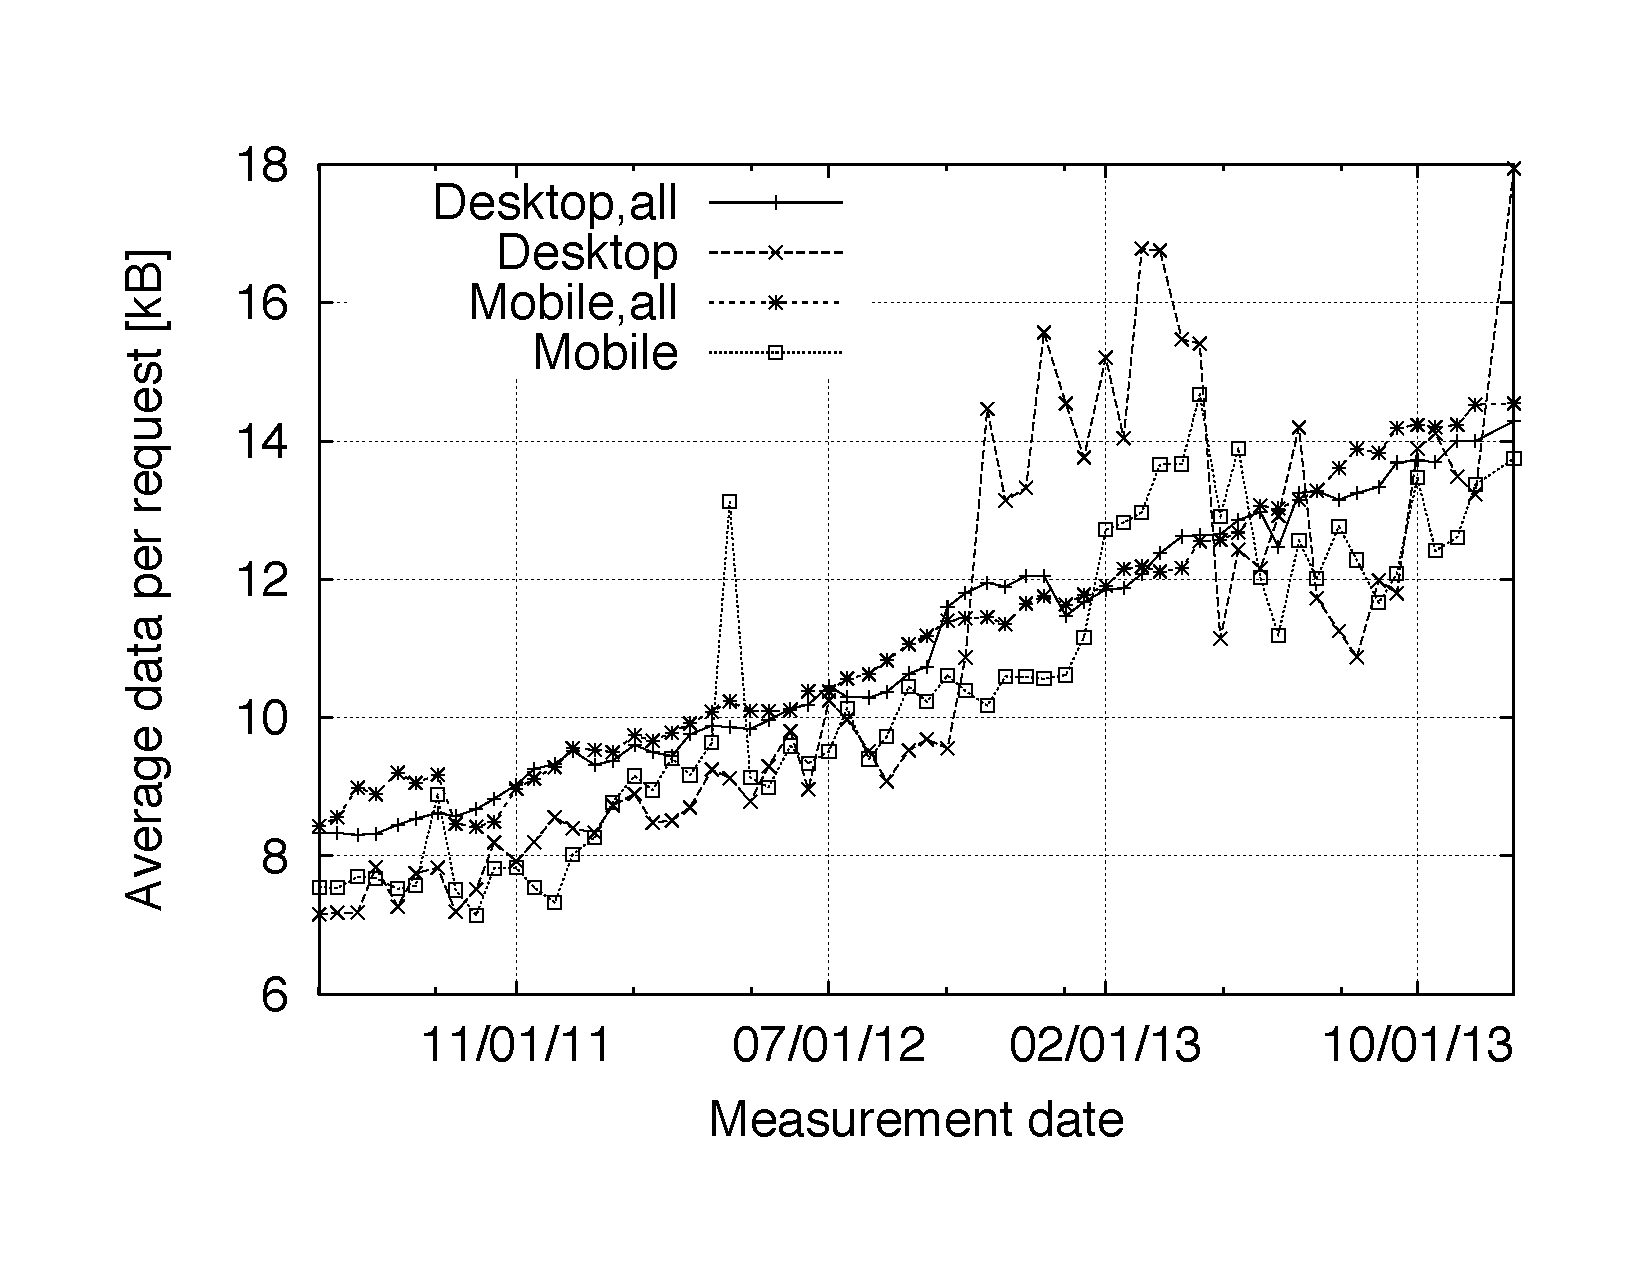
\includegraphics[width=.45\textwidth]{bpr_all}}\\
	\subfloat[Categorized for desktop client (all pages).]{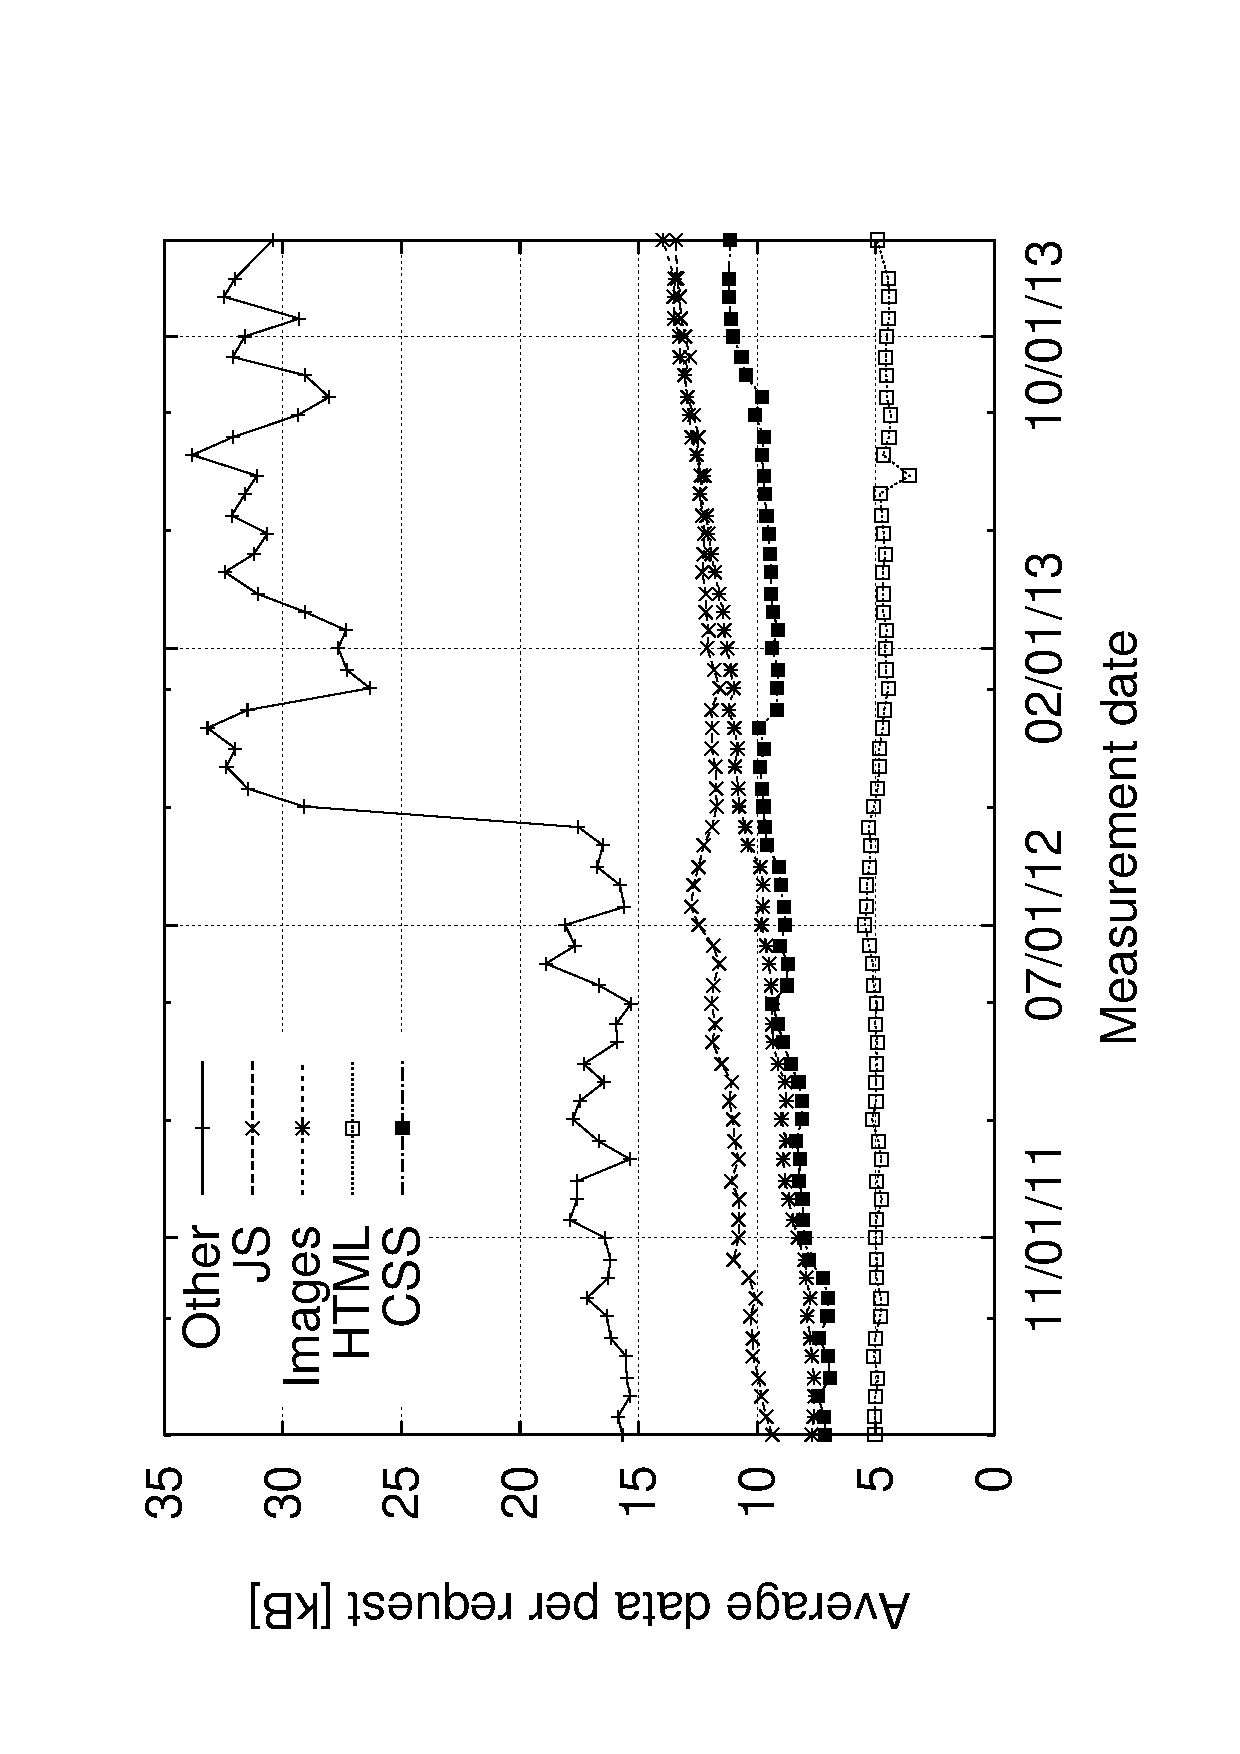
\includegraphics[width=.45\textwidth]{bpr_by_type_fixed_all}}\qquad
	\subfloat[Categorized for  mobile client (all pages).]{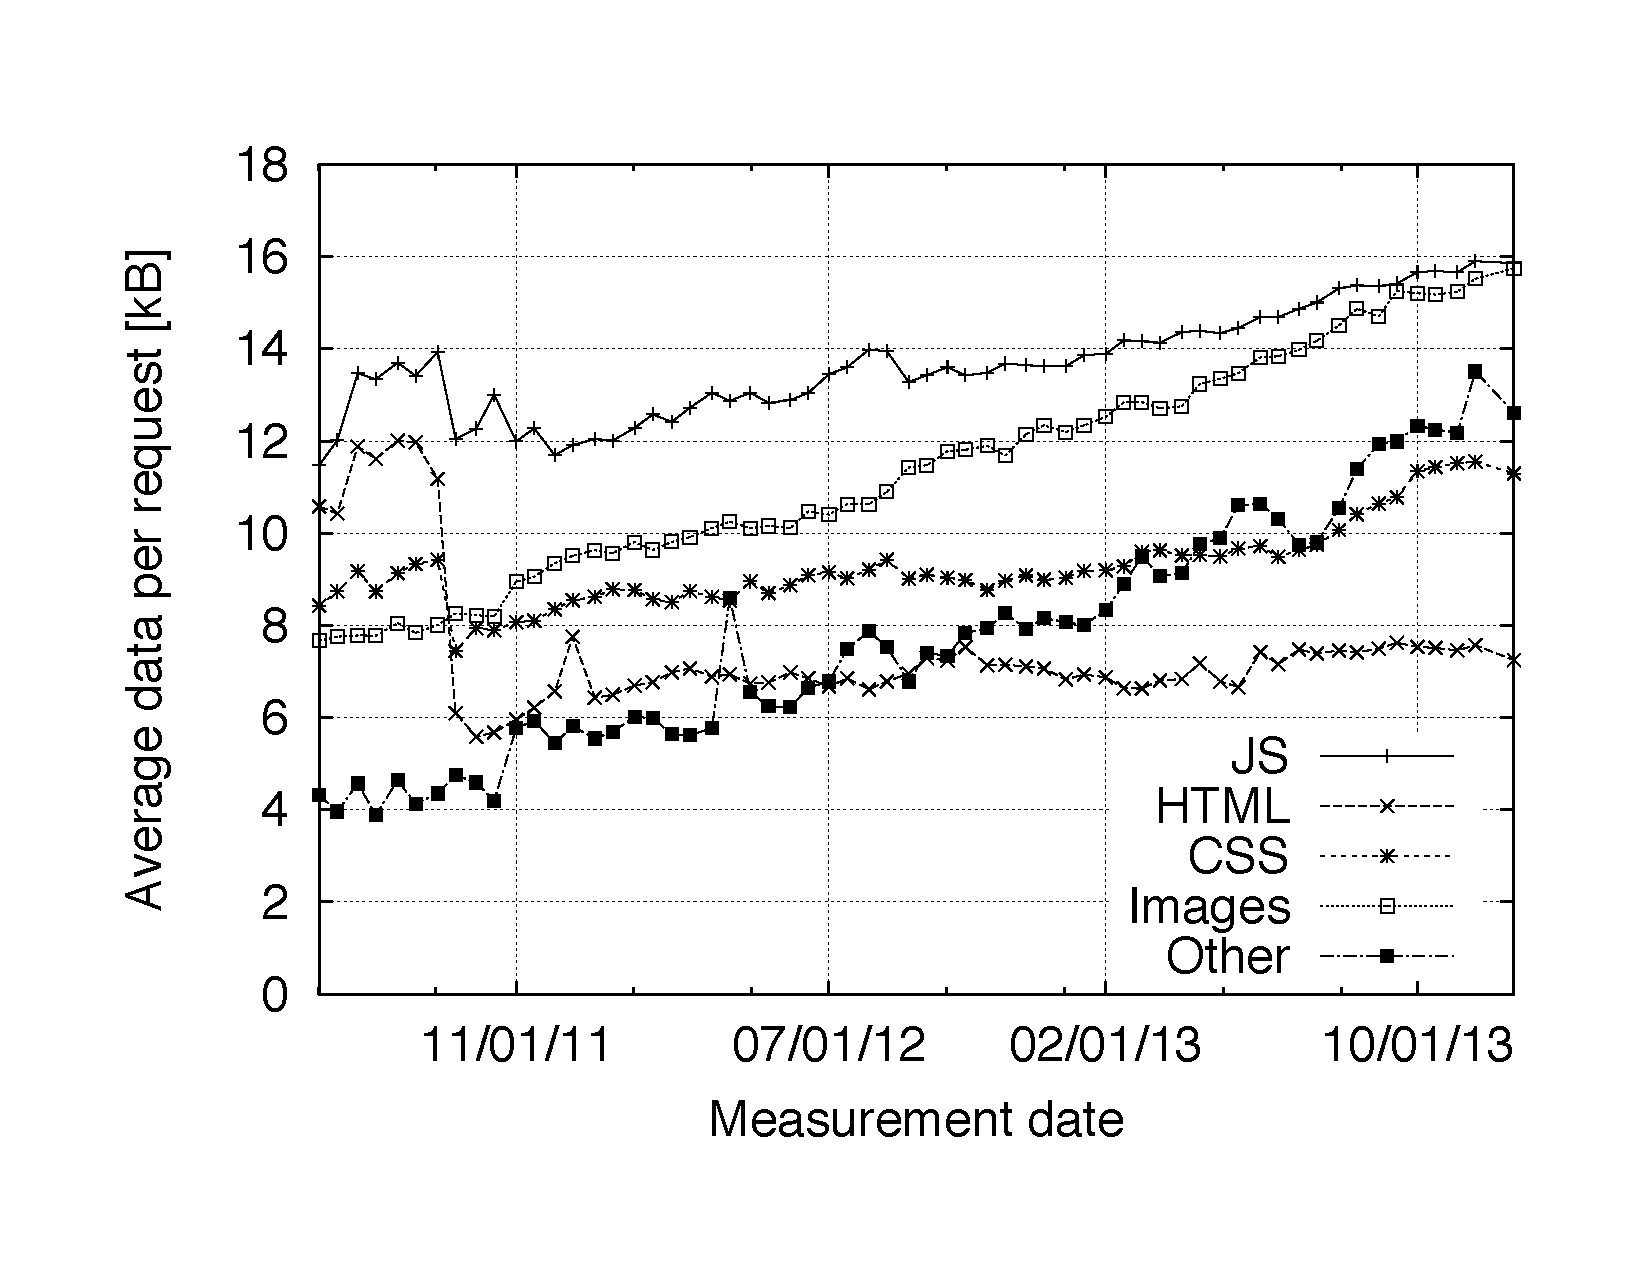
\includegraphics[width=.45\textwidth]{bpr_by_type_mobile_all}}
	\caption{Average number of bytes per web page object request for desktop and mobile versions and decomposition into  HTML, CSS, Java Script, Images, and Other object categories.\label{fig:relative}}
\end{figure}
For the average number of bytes per web page request, illustrated in Figure~\ref{fig:relative}~(a), we note a steady increase for both desktop and mobile client requests. 
In greater detail, we note that the overall trend for both request origins is rather linear and close.
In turn, we note that both feature an almost identical overall growth rate of about 0.9\% every two weeks.
Verifying these original findings by comparing them with the smaller size subset of web pages, we note that even these pages exhibit the same underlying trend, albeit in conjunction with increased variability.
This is a finding with great long-term implications for simplified approaches to modeling, e.g, in capacity determination scenarios.

Next, we investigate the behavior more closely by evaluating the HTML, CSS, Java Script, Images, and Other categories separately for the desktop and mobile clients in Figures~\ref{fig:relative}~(b) and \ref{fig:relative}~(c), respectively.
For desktop requests, we note that the highest number of bytes per request can be observed for the Other category, with a pronounced ``jump'' in the time frame of base URL adjustments in the underlying dataset. 
In turn, we reason that more components, such as Flash or font data, are included in the larger underlying set of web pages evaluated, which results in the current level of around 33 kB per request in this category.
For Java Script and CSS data per request, we observe  initially growing trends, which have slowed over time and now are moving beyond 14 and 11 kB, respectively.
Images, on the other hand, continue their growing trend and now feature about 14 kB per request.
The actual HTML markup request size has remained relatively constant at around 5 kB.
For requests from mobile clients, on the other hand, we note that the largest amount per request is observed for Java Script, with currently growing sizes above 15 kB.
The Images and Other categories also feature a significant growth for mobile client requests, which have risen above 15 and 12 kB, respectively.
The HTML and CSS categories are fairly stable with only minimal growth over time, which is similar to the trends observed for the desktop clients.

In comparison, we note that while both average client request sizes are comparable with respect to their level and growth rates, the actual composition is significantly different. 
While desktop request sizes are mainly determined by the Other category data, such as Flash or fonts, and increasingly images, mobile requests are mainly characterized by Java Script and Images.
The reason behind this behavior could be the increased level of rich media inclusion for desktop clients (e.g., using Flash), whereas automatic adjustments performed (e.g., using Java Script) disable this for mobile clients, where this is not desired. 
Furthermore, we note that the average amount of bytes per image is fairly close (even a bit higher for mobile), which could be due to increased utilization of content management systems.
These commonly utilized frameworks typically adjust web page layouts and theming elements based on the requesting client, e.g., format for mobile display sizes and utilize smaller sized theming elements. The actual main content elements, however, typically remain unchanged (which, in turn, results in identical downloads of the larger sized content images).

\subsection*{Caching of Web Page Objects}
\addcontentsline{toc}{subsection}{Caching of Web Page Objects}
One of the main assumptions for the prior evaluation was that the data represents ``first views,'' i.e., the dataset's underlying measurements do not consider the caching of web pages after initial visits. 
The individual entries in the datasets obtained from httparchive.org, however, additionally contain the max-age header (amongst other, such as expiration) directives for evaluation of the maximum lifetime of objects on the requesting device. The locally cached data can have a positive impact on the required network access, especially for mobile devices.
We illustrate the different max-age values obtained from the data in Figure~\ref{fig:maxage}~(a) for desktop client requests.
\begin{figure}
	\centering
	\subfloat[Desktop clients]{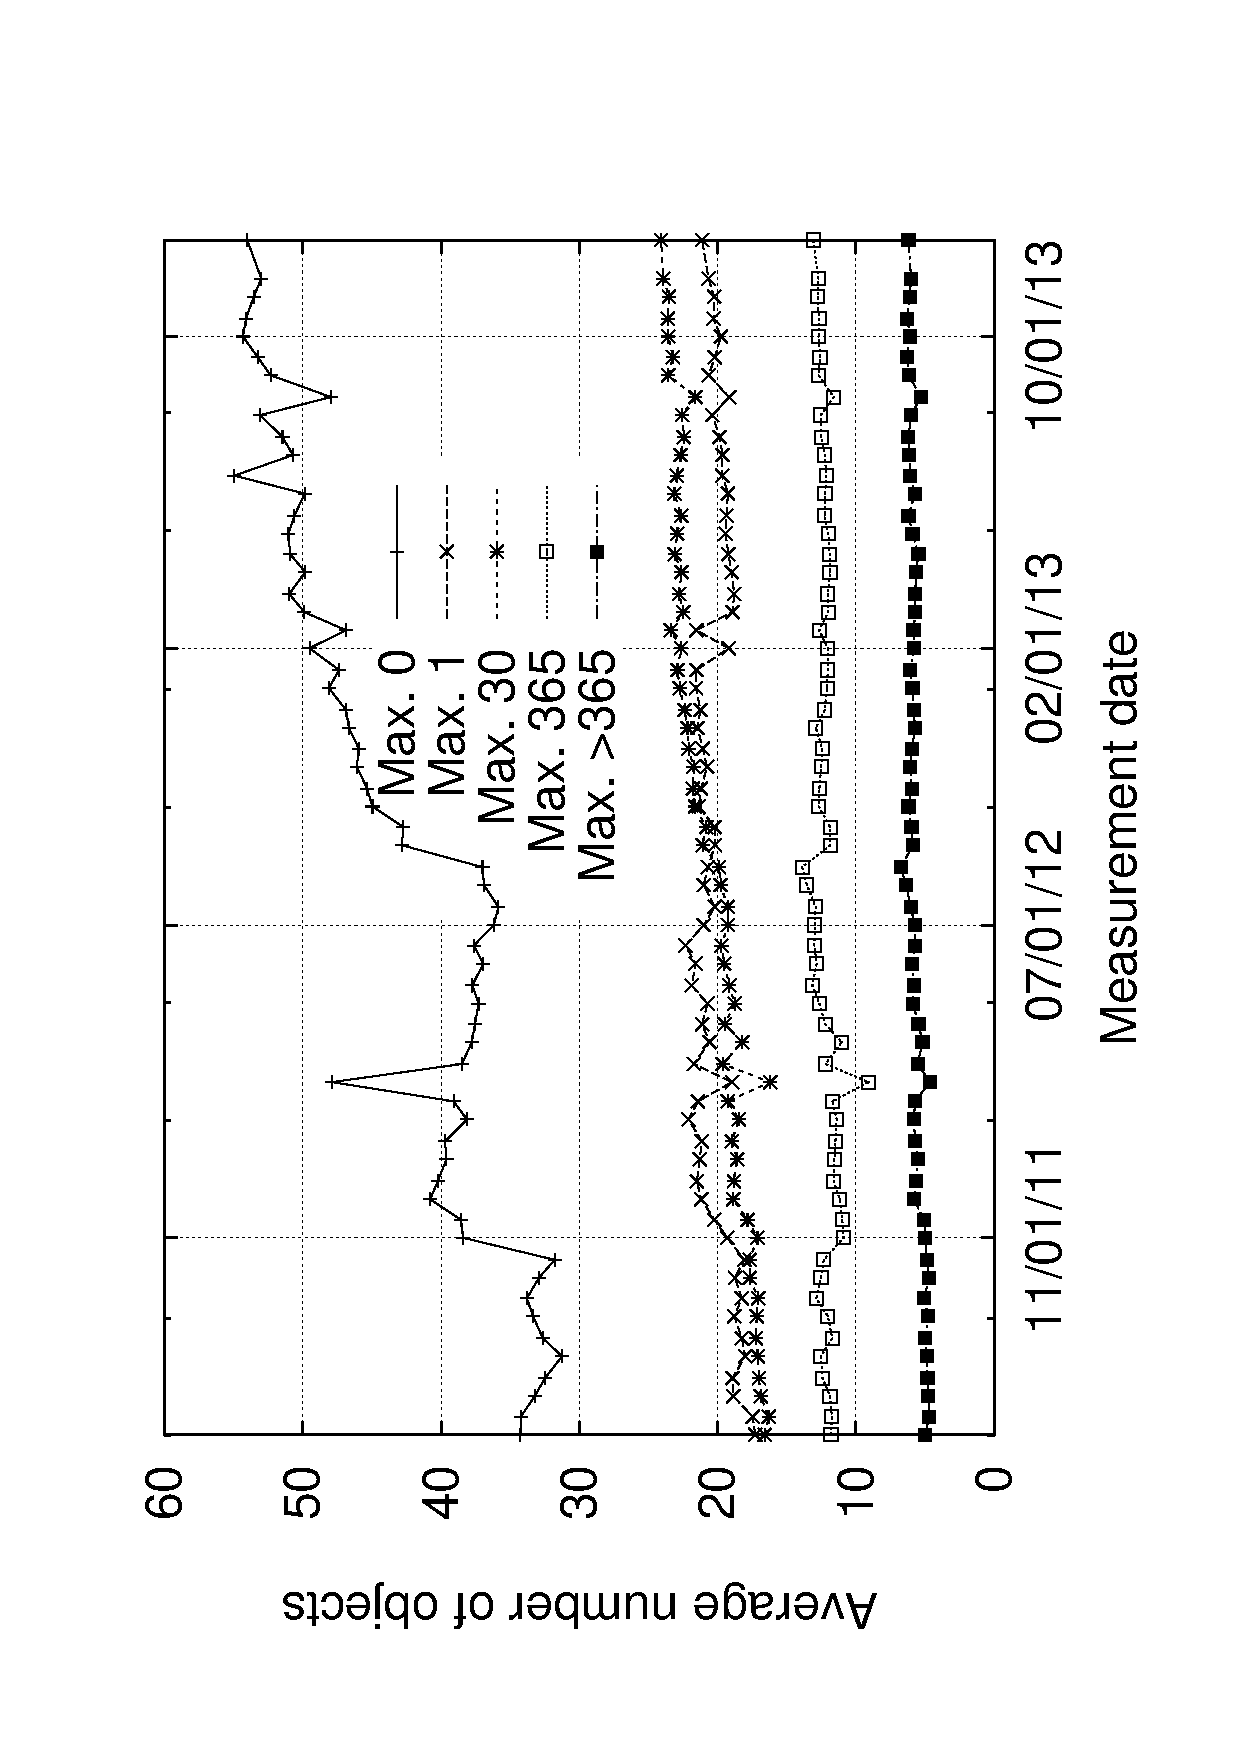
\includegraphics[width=.45\textwidth]{cache_fix_all}}\qquad
	\subfloat[Mobile clients]{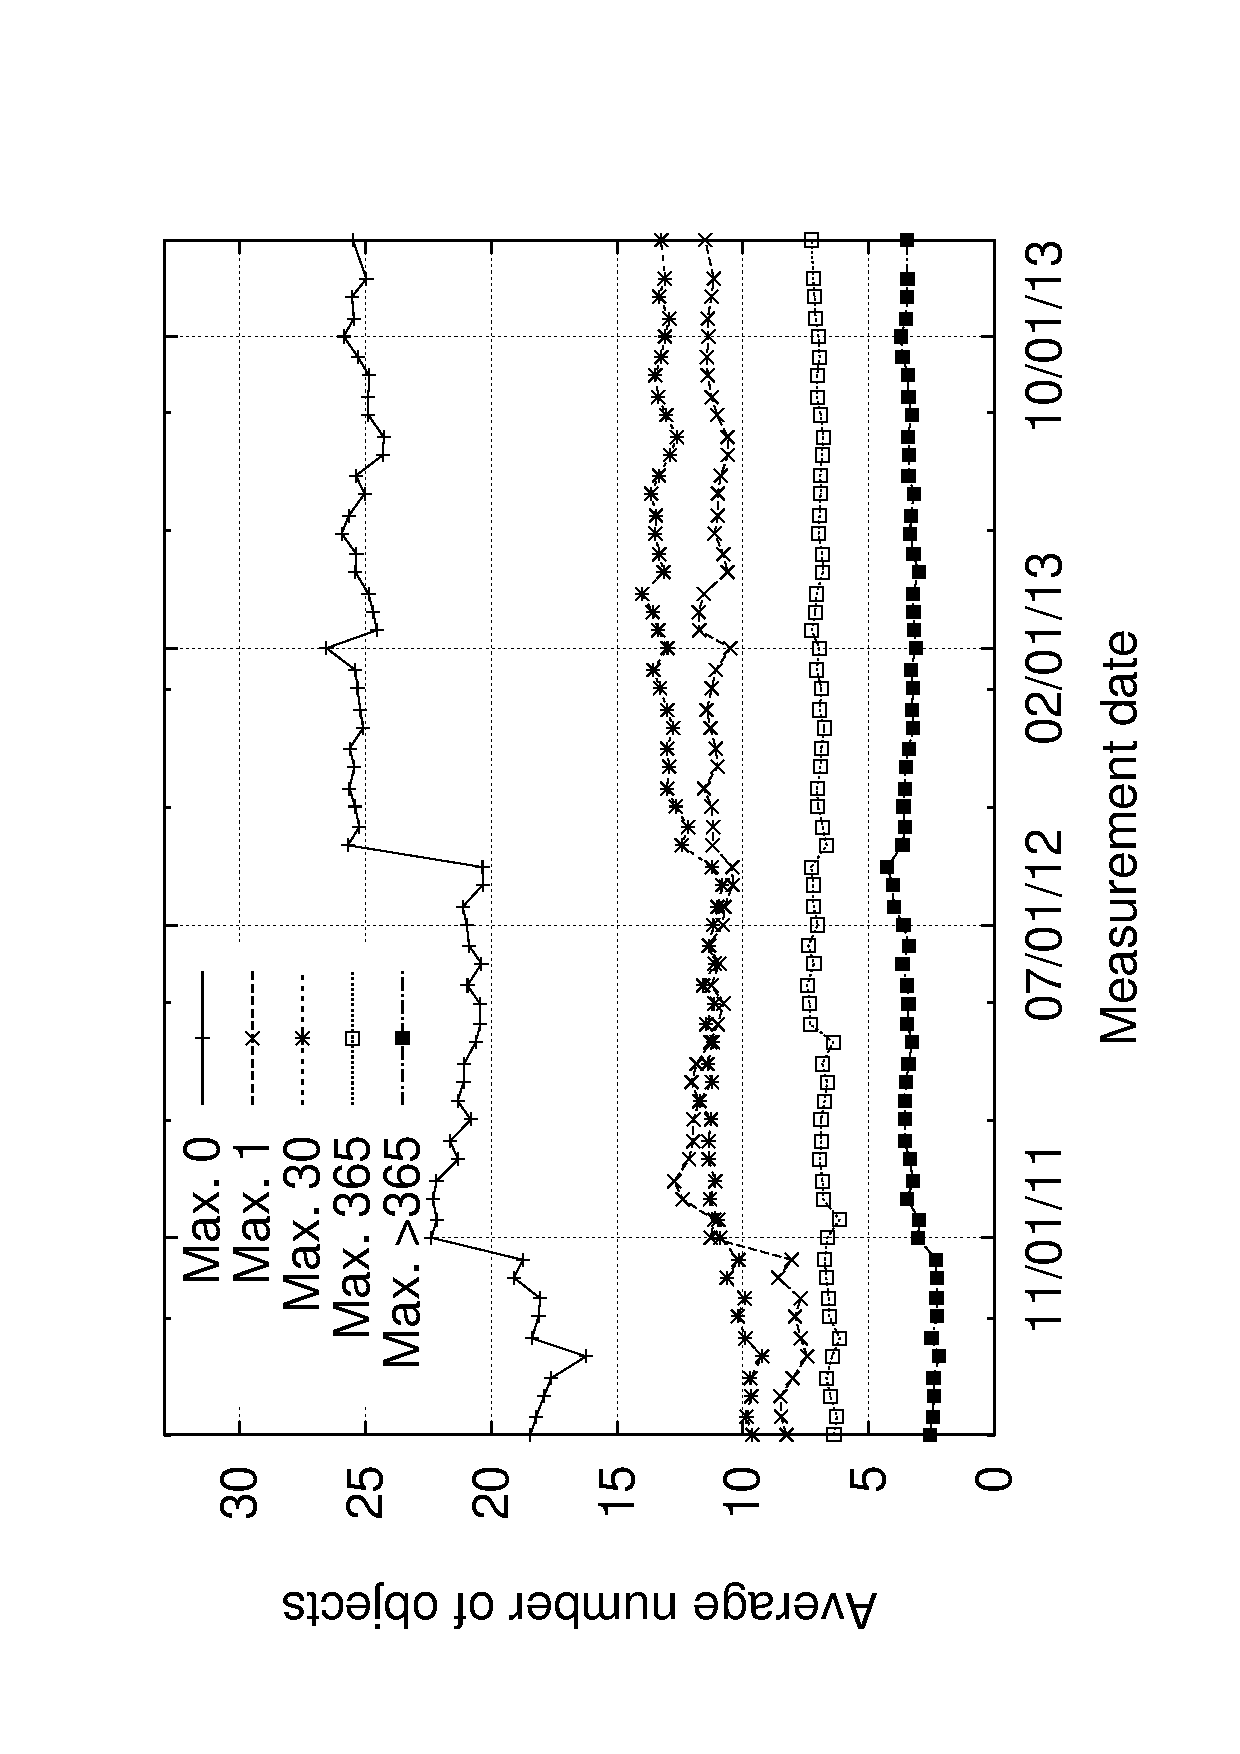
\includegraphics[width=.45\textwidth]{cache_mob_all}}\\
	\caption{Maximum age of web page objects for desktop and mobile web clients.\label{fig:maxage}}
\end{figure}
We observe that the largest fraction of items cannot be cached beyond a day, and in turn requires frequent downloads if web pages are visited infrequently. 
More importantly, this is the only category that exhibits significant continued growth.
Over the time horizon we consider here, items that are stored between one and up to 30 days can be considered regularly downloaded at a comparable level, while only a relatively small number of objects can be considered invariant due to larger maximum allowable cache ages.
For the mobile client counterparts illustrated in Figure~\ref{fig:maxage}~(b), we initially note a similar level and continued growth for the average number of objects that are able to be cached below a day (considering the overall average number of objects requested as discussed in Section~\ref{ss:objects}).
Objects that require regular, but less frequent downloads as well as more invariant items follow the trends observed for the desktop client.
Overall, the implication for mobile clients is that the fraction of requests with a shorter cache lifetime constitutes the majority of requests and in turn will require frequent downloads if web pages are visited infrequently.


\section*{Implications}
\addcontentsline{toc}{section}{Implications}
\label{s:discuss}
One initial limitation of our dataset is the evaluation of landing pages only, which, however, could be seen as an actual upper limit, according to \cite{BuMaSe13}. 
Overall, we find significantly growing trends for the average web page number of objects and their sizes.
The immediate implications from the growing trend of the number of web request per fixed and mobile website versions and their respective size is that the pressure on access networks capacity growths will continue, see, e.g., \cite{Ci13} for a detailed separation into typical business and consumer categories of accesses Internet data.
We find significant similarities between the desktop and the mobile versions of the popular web pages that were part of this evaluation. 
Mobile counterparts of desktop page versions typically feature less objects and smaller sizes; both characteristics typically also exhibit a significantly slower growth.
As briefly outlined by the authors of \cite{BuMaSe13}, the reduced number of servers and number of objects involved likely can be seen as an indicator of the correlation between the two different versions of popular web pages.

As previously outlined in~\cite{ThAgNiBoSi12}, Java Script objects in mobile web pages are a main contributor to the rendering power consumption, and we find significant amounts of Java Scripts to be contained in average web pages.
More importantly, we conceive that there is a significant amount of data and requests in average mobile pages that is dedicated to image and other objects, which will contribute significantly to the combined transmission and rendering energy costs, as outlined in \cite{ThAgNiBoSi12} as well.
Optimization efforts that target mobile clients specifically should in turn focus on these categories of data, specifically while taking more advantage of caching possibilities, as the transmission energy contributes a significant amount to the total energy required.
%
% Correlation
%
Combining the two prior evaluation categories, the average total number of bytes per request for desktop and mobile web pages are very similar and exhibit a linearly growing trend.
This finding for the larger dataset is additionally corroborated by evaluation of the continuously present web pages, which exhibit the same trend, albeit at higher levels of variability.
While some of the greater details highlight smaller differences by respective type of object requested, the overall direct correlation between the two gives rise to future research questions.
%
% Comparison
%
Comparing our results with prior longitudinal studies in \cite{CaAlPa10,IhPa11}, we note several interesting similarities and other findings, within the constraints given by each of the three studies.
First, both prior studies cover date ranges prior to our study's time frame, ending in 2009 and 2010, respectively. They are based on actual user request analyses derived from proxy monitoring, whereas our study specifically utilizes an evaluation of the landing pages of popular web sites, which can be regarded as more static.
The HTTP GET transaction size evaluation performed in \cite{CaAlPa10}, which is also corroborated by the median page size growth ending around 133 kB reported in \cite{IhPa11}, provides an almost seamless trend continuation over time (especially when considering the different study parameters, which include follow-up session browsing).

As indicated by \cite{IhPa11} for prior years, our study also finds a significant shift in the bytes per object -- with  images constituting the majority of traffic in both request scenarios.
In the recent years we evaluate, however, we now note a shift to the desktop client's Other category, while mobile clients exhibit a significantly smaller overall size and lower amounts of data in the Other category.
Comparing initial caching observations here with the results provided in  \cite{CaAlPa10,IhPa11}, we note that the overall number of cacheable objects is increasing for the desktop requests, which is in line with the GET request savings described in \cite{CaAlPa10}, where about 20-25\% were identified.
Similarly, \cite{IhPa11} reports 27-37.1 \% of objects to fall into this category for US-based traffic, resulting in byte savings of 16.8-28.1\%.
In turn,  the cache-based object retrieval can reduce the waiting times to amounts that fall within positive user experience time frames, see, e.g., \cite{NiUeNa10}.
In conclusion, our study finds a continuation of prior longitudinal studies when overall trends are regarded, but differences in the lower-level shifts of requests and data by categories and requesting device.

\section*{Conclusion}
\addcontentsline{toc}{section}{Conclusion}
\label{s:conc}
This overview represents the first longitudinal and comparative study of the current state and changes of the World Wide Web, as seen by current fixed and mobile clients when requesting web pages.
We utilized the publicly available data from httparchive.org, an industry-supported web page statistics archival project, to outline major trends and resulting implications.
For the number of web-page requests, we noted an overall growing trend, with a slightly higher rate for desktop versions of web pages, continuing trends observed in the past. 
Modern web desktop page versions feature well above 100 object requests on first views, while mobile versions trail above 60.
Similarly, we noted a rapidly increasing trend with regard to the average web page sizes, with desktop pages surpassing 1.5 MB in initial view size, while mobile pages trail at more than 50\%.
Most astonishingly, this study found that the average bytes per request are within close proximity for fixed and mobile clients and exhibit both comparable as well as significant growth rates.
When performing decomposition into categories, we found that Image, Other (such as Flash or fonts), and Java Script objects are the main contributors to web page sizes for both clients. Furthermore, the most requests for objects on first view are attained for the Image category of web page objects, again independent of the client type.
We also evaluated the potential of caching objects for subsequent views of web pages, whereby we found that most web page objects exhibit very short cache life times of a one day maximum.
Our overview thus suggests that there are significant opportunities for future research and optimization efforts for efficient mobile web content delivery. 
Specifically, our findings indicate the need for more optimization and client considerations when designing modern web pages and frameworks that are utilized for their delivery.
